\documentclass[12pt]{article}
\usepackage{amsmath}
\usepackage[UTF8]{ctex}
\usepackage{ytableau}
\usepackage{tikz}
\usepackage{wrapfig}
\usepackage{geometry}

\geometry{left=2.0cm,right=2.0cm,top=2.0cm,bottom=2.0cm}

\newtheorem{definition}{定义}[subsection]
\newtheorem{theorem}{定理}[subsection]
\newtheorem{proof}{证明}[subsection]
\newtheorem{corollary}{推论}[subsection]
\newtheorem{example}{例}[subsection]

\begin{document}
    \title{二次量子化笔记}
    \author{中科院物理所\\李成蹊}
    \maketitle
    \section{置换群与全同粒子}
    \subsection{置换}
    n个客体排列次序的变换称为置换,n个客体一共有$n!$个不同的置换。置换可以用$2\times n$矩阵来描述
    \begin{equation*}
        R=\begin{pmatrix}
            1&2&\cdots&j&\cdots&n\\
            r_1&r_2&\cdots&\r_j&\cdots&r_n
        \end{pmatrix}
    \end{equation*}
    例如置换群元素$R$作用在基函数$\Psi=(\varphi_1\,\varphi_2\,\varphi_3),R=\begin{pmatrix}
        1&2&3\\
        2&3&1
    \end{pmatrix}$得到
    \begin{equation*}
        R\Psi=\begin{pmatrix}
            1&2&3\\
            2&3&1
        \end{pmatrix}(\varphi_1\,\varphi_2\,\varphi_3)=(\varphi_3\,\varphi_1\,\varphi_2)
    \end{equation*}
    置换乘法的定义为相继做两次置换,在这个定义上,置换构成群。

    有一类特殊的置换,$n-l$个客体保持不变,$l$个客体顺序变换,形成一个循环,$l$称为轮换长度。
    \begin{equation*}
        (a_1\,a_2\,\cdots\,a_l)=\begin{pmatrix}
            a_1&\cdots&a_{l-1}&a_l&b1&\cdots&b_{n-l}\\
            a_2&\cdots&a_l&a_1&b_1\cdots&b_{n-l}
        \end{pmatrix}
    \end{equation*}
    用行矩阵描述轮换,数字排列次序不能改变,但可以顺序变换
    \begin{equation*}
        (a\,b\,c\cdots\,p\,q)=(b\,c\,\cdots\,p\,q\,a)
    \end{equation*}
    长度为1的轮换是恒等变换,长度为2的轮换称为对换,对换满足
    \begin{equation*}
        (a\,b)=(b\,a),\quad(a\,b)^2=E
    \end{equation*}
    长度为$l$的轮换它的$l$次自乘等于恒元,即它的阶数为$l$。没有公共客体的轮换,乘积次序可以交换。

    任何一个置换都可以唯一地分解为没有公共客体的轮换乘积。例如
    \begin{equation*}
        R=\begin{pmatrix}
            1&2&3&4&5\\
            3&4&5&2&1
        \end{pmatrix}=(1\;3\;5)(2\;4)=(2\;4)(1\;3\;5)
    \end{equation*}
    把置换分解为没有公共客体的轮换乘积时,各轮换长度的集合称为该轮换的轮换结构。例如上例
    \begin{equation*}
        R=(1\;3\;5)(2\;4)\text{轮换结构为$(3,2)$}
    \end{equation*}
    把一个正整数$n$分解成若干个正整数之和,这样的正整数的集合称为$n$的一族配分数。例如:
    \begin{enumerate}
        \item $n=2$时可能的配分数为$(2),(1^2)$
        \item $n=3$时可能的配分数为$(3),(2,1),(1^3)$
    \end{enumerate}
$n$个客体任意置换的轮换结构由一族配分数来描写:$(l_1,l_2,\cdots),\sum_il_i=n$
\subsection{置换群的类与生成元}
我们知道一个元素的共轭元素为$SRS^{-1}$,把$R$置换的上下两行数字同时做$S$置换得到$R$置换的共轭元素$SRS^{-1}$。例如
\begin{equation*}
    S(a\;b\;c\;\cdots\;d)S^{-1}=(s_a\;s_b\;\cdots\;s_d)
\end{equation*}
共轭不改变轮换长度,只改变轮换的客体编号。互相共轭的两个置换轮换结构相同。

设$R=(a_1\;a_2\;a_3)(b_1\;b_2)\cdots(c_1\;c_2\;\cdots\;c_l)\quad R'=(d_1\;d_2\;d_3)(e_1\;e_2)(f_1\;f_2\;\cdots\;f_l)$

存在$S=\begin{pmatrix}
    a_1&a_2&a_3&b_1&b_2&\cdots&c_1&c_2&\cdots&c_l\\
    d_1&d_2&d_3&e_1&e_2&\cdots&f_1&f_2&\cdots&f_l
\end{pmatrix}\in S_n$

使得$SRS^{-1}=R'$
有相同轮换结构的两个置换必定相互共轭。所以置换群的类可以用轮换结构来描写,置换的轮换结构则用配分数来描写。置换群的类数等于整数$n$分解为不同配分数的数目。

如果置换群$S_n$的类包含$\nu_1$个1循环,$\nu_2$个2循环,$\cdots$,$\nu_n$个n循环,即它的轮换结构为
\begin{equation*}
    (l)=(1^{\nu_1},2^{\nu_2},\cdots,n^{\nu_n}),\quad \nu_1+2\nu_2+\cdots+n\nu_n=n
\end{equation*}
类所包含的元素个数为
\begin{equation*}
    C_l=\frac{n!}{1^{\nu_1}2^{\nu_2}\cdots n^{\nu_n}\nu_1!\nu_2!\cdots\nu_n!}
\end{equation*}
在轮换每一客体处切断,轮换会分解为对换的乘积。一般地,长度为l的轮换可以分解为l-1个对换的乘积,即
\begin{equation*}
    (a\;b\;c\cdots t\;p\;q)=(a\;b)(b\;c)\cdots(t\;p)(p\;q)
\end{equation*}
任何置换都可以分解为若干对换的乘积,分解方式虽然不唯一,但包含对换个数的奇偶性是确定的:轮换长度确定了对换个数的奇偶性。置换分解为对换乘积时,对换数目是偶数的置换称为欧置换,对换数目是奇数的置换称为奇置换。
\begin{enumerate}
    \item 恒元是偶置换
    \item 偶置换乘奇置换为奇置换
    \item 两个偶置换或两个奇置换相乘为偶置换
\end{enumerate}
置换群所有偶置换的集合构成指数为2的不变子群,称为交变子群,奇置换的集合是陪集,商群$C_2$。商群的群表示是原群的非真实表示,所以$n>1$时,$S_n$除恒等表示以外,还有一维非恒等表示,叫做反对称表示,表示矩阵的值叫做表示置换宇称,记作
\begin{equation*}
    \delta(R)=\begin{cases}
        1\quad&\text{当$R$是偶置换}\\
        -1\quad&\text{当$R$是奇置换}
    \end{cases}
\end{equation*}
为了方便,我们将不同客体之间的对换记作$P_{a\,b}=(a\;b)$。任何置换都可以约化成无公共客体轮换的乘积,任何轮换都可以分解成若干对换的乘积,而任何对换都可以表示为相邻客体的对换乘积,例如
\begin{equation*}
    \begin{split}
        P_{a\,a+k}&=P_{a+1\,a+k}P_{a\,a+1}P_{a+1\,a+k}^{-1}\\
        P_{a+1\,a+k}&=P_{a+2\,a+k}P_{a+1\,a+2}P_{a+2\,a+k}^{-1}
    \end{split}
\end{equation*}
依次迭代下去,任何置换都可以表示为相邻客体的对换乘积。

引入长度为$n$的轮换$W=(1\;2\;\cdots\;n)$,则有
\begin{equation*}
    P_{a\,a+1}=WP_{a-1\,a}W^{-1}=W^2P_{a-2\,a-1}W^{-2}=\cdots=W^{a-1}P_{1\,2}W^{-(a-1)}
\end{equation*}
任何相邻客体的对换都可由$W$和$P_{1\,2}$生成。所以置换群的生成元是$W$和$P_{1\,2}$,秩为2
\subsection{杨图杨表杨算符}
\subsubsection{杨图和杨表}
有限群不等价不可约表示个数等于类的数目。置换群$S_n$的类可以用配分数来表述,值得注意配分数描写的类和不可约表示没什么关系。

任取一组配分数$[\lambda]=[\lambda_1,\lambda_2,\cdots,\lambda_m]$
\begin{equation*}
    \lambda_1\geq\lambda_2\geq\cdots\geq\lambda_m>0,\quad\sum_{j=1}^m\lambda_j=n
\end{equation*}
画一个n格的方格图,分成$m$行,左边对齐,第一行$\lambda_1$个格子,第二行$\lambda_2$个格子,依次下去。这样画出来的图称为杨图。我们把格子数从上到下,从左到右依次增加的图叫正则杨图。

定义杨图的大小:对于两个杨图,由第一行开始比较它们的格子数,第一次出现格子数不同时,格子大的杨图大于格子小的杨图。例如$S_3$群杨图从大到小排列为
\begin{center}
    \hbox to \hsize{\vbox{\hsize=0.3\hsize \ydiagram{3}}\vbox{\hsize=0.3\hsize \ydiagram{2,1}}\vbox{\hsize=0.3\hsize \ydiagram{1,1,1}}}
\end{center}
$[3]>[2,1]>[1^3]$

每个杨图都唯一对应于置换群$S_n$的一个不可约表示,不同杨图对应的不可约表示不等价。

杨图$[\lambda]$的行和列互换得到的杨图$[\tilde{\lambda}]$称为杨图$[\lambda]$的对偶杨图,对应的不可约表示称为对偶表示。若杨图$[\lambda]=[\tilde{\lambda}]$则称为自偶杨图

对于给定杨图$[\lambda]$,把1到n的n个自然数分别填入杨图的n个格子中,就得到一个杨表。n个格子的杨图对应有n!个杨表,只有那些在杨表的每一行从左往右从上到下依次递增的杨表叫做正则杨表。

同样的可以定义正则杨表的大小:同一个杨图对应的正则杨表,从第一行开始逐行从左往右开始比较他们的填数。第一次出现填数不同时,填数大的正则杨表大。例如杨图$[3,2]$的杨表大小顺序,从小到大为
\begin{center}
\ytableausetup
{mathmode, boxsize=1.5em}
\begin{ytableau}
    1&2&3\\
    4&5
\end{ytableau}<
\begin{ytableau}
    1&2&4\\
    3&5
\end{ytableau}<
\begin{ytableau}
    1&2&5\\
    3&4
\end{ytableau}<
\begin{ytableau}
    1&3&4\\
    2&5
\end{ytableau}<
\begin{ytableau}
    1&3&5\\
    2&4
\end{ytableau}
\end{center}
杨图$[\lambda]$对应的不可约表示的维数或正则杨表个数由钩子定理给出:

\begin{wrapfigure}{r}{2cm}
    \centering
    \includegraphics[width=1in]{fig1.png}
    \caption{\footnotesize 钩子路径}
\end{wrapfigure}
对杨图的第i行第j列格子,定义钩形数$h_{ij}$,它等于一条钩形路径在杨图中经过的格子数,这条路径从杨图第i行最右面的格子处进入杨图,向左走到第i行第j列格子处向下转弯,从第j列最下面的格子处离开杨图。把每个格子对应的钩形数填入杨图中得到钩形数表,用总的排列数n!除以钩形数乘积就是杨图$[\lambda]$对应的杨表个数。
\begin{equation*}
    d_{[\lambda]}=\frac{n!}{\prod_{ij}h_{ij}}
\end{equation*}
可以看到所有$n$格杨图正则杨表数的平方和正好等于$n!$
\begin{equation*}
    \sum_{[\lambda]}[d_{[\lambda]}(S_n)]^2=n!
\end{equation*}
\subsubsection{杨算符}
横向置换:对于给定杨表同行客体的置换,第j行横向置换$P_j$共有$\lambda_j!$个,横向置换的乘积还是横向置换。
横算符:所有横向置换之和称为横算符$\mathcal{P}$
\begin{equation*}
    \mathcal{P}=\sum P=\sum\prod_{j}P_j=\prod_{j}[\sum P_j]
\end{equation*}
同样的,定义纵向置换:同列数字间的置换称为该杨表的纵向置换。若杨图第k列有$\tau_k$格子,则第$k$列总想置换$Q_k$共有$\tau_k$个
纵算符:所有纵向置换$Q$乘以它的置换宇称$\delta(Q)$后相加,称为该杨表的纵算符$\mathcal{Q}$
\begin{equation*}
    \mathcal{Q}=\sum\delta(Q)Q=\sum\prod_{k}\delta(Q_k)Q_k=\prod_{k}[\sum\delta(Q_k)Q_k]
\end{equation*}
对于给定杨表,横算符和纵算符的乘积称为该杨表的杨算符$\mathcal{Y}$

例如计算杨表
\ytableausetup{mathmode,boxsize=1.2em}
\begin{ytableau}
    1&2&3\\
    4&3
\end{ytableau}的杨算符
\begin{equation*}
    \begin{split}
        \mathcal{Y}&=\{E+(12)+(13)+(23)+(123)+(321)\}\{E+(45)\}\{E-(14)\}\{E-(25)\}
    \end{split}
\end{equation*}
在具体写出横算符时,通常先把每一行的所有横向置换加起来,然后把不同行的横向置换之和乘起来。同样的,具体写出纵算符时,先把每一列的所有总想置换乘上各自的置换宇称后相加,然后把不同列的纵向置换的代数和乘起来。

由于置换群的共轭关系是改变置换客体,若置换$S$把杨表$\mathcal{Y}$变成杨表$\mathcal{Y}'$,则相应的杨算符满足共轭关系$\mathcal{Y}'=S\mathcal{Y}S^{-1}$。例如
\begin{center}
    \ytableausetup{mathmode,boxsize=1.2em}
    杨表$\mathcal{Y}=$
    \begin{ytableau}
        1&3&5\\
        2&4
    \end{ytableau}
    ,杨表$\mathcal{Y}'$=
    \begin{ytableau}
        1&2&3\\
        4&5
    \end{ytableau}
    ,$S=
    \begin{pmatrix}
        1&3&5&2&4\\
        1&2&3&4&5
    \end{pmatrix}$
    \begin{equation*}
        S\mathcal{Y}S^{-1}=\mathcal{Y}',\quad S\mathcal{P}S^{-1}=\mathcal{P}',\quad S\mathcal{Q}S^{-1}=\mathcal{Q}'
    \end{equation*}
\end{center}
杨算符是置换群元素的代数和,也是置换群群代数的矢量。
\begin{equation*}
    \mathcal{Y}=\sum_{R\in S_n}F(R)R
\end{equation*}
这里群代数矢量展开系数$F(R)$只能取1,-1,0. 横向置换恒元系数为1,纵向置换$Q$和PQ的系数为Q的置换宇称$\delta(Q)$.

这里介绍几个杨算符的性质
\begin{enumerate}
    \item 杨算符对于左乘横向置换保持不变,对右乘纵向置换产生一个宇称因子$\delta(Q)$
    \begin{equation*}
        P\mathcal{Y}=\mathcal{Y},\quad Q\mathcal{Y}=\delta(Q)\mathcal{Y}
    \end{equation*}
    \item 若$T_0$同时是杨算符$\mathcal{Y}=\mathcal{PQ}$的横向对换和杨算符$\mathcal{Y}'=\mathcal{P}'\mathcal{Q}'$的纵向对换,则有
    \begin{equation*}
        \mathcal{Y}'\mathcal{Y}=0
    \end{equation*}
    证明很简单$\mathcal{Q}'\mathcal{P}=\mathcal{Q}'T_0\mathcal{P}=-\mathcal{Q}'\mathcal{P}=0$
    \item 若杨图$\mathcal{Y}'<\mathcal{Y}$,则杨算符$\mathcal{Y}'$左乘杨算符$\mathcal{Y}$得零
    \begin{equation*}
        \mathcal{Y}'\mathcal{Y}=0,\quad \mathcal{Y}'<\mathcal{Y}
    \end{equation*}
    证明利用性质2显然可以得到
    \item 对同一个杨图,若正则杨表$\mathcal{Y}'$大于正则杨表$\mathcal{Y}$,则杨算符$\mathcal{Y}'$左乘杨算符$\mathcal{Y}$得零
    \begin{equation*}
        \mathcal{Y}'\mathcal{Y}=0,\quad \mathcal{Y}'>\mathcal{Y}
    \end{equation*}
    \item 对于同一个杨图,设填在杨表$\mathcal{Y}'$同一列数字的都不在杨表$\mathcal{Y}$的同一行,则把杨表$\mathcal{Y}$变成杨表$\mathcal{Y}'$的置换$R$满足$R\in\mathcal{Y},R\in\mathcal{Y}'$
    \item 置换群元素$R\notin\mathcal{Y}$的充要条件是
    \begin{equation*}
        R=P_0RQ_0
    \end{equation*}
    其中$P_0,Q_0$分别是杨表$\mathcal{Y}$的某一个横向对换和纵向对换
\end{enumerate}
\subsubsection{置换群的幂等元}
置换群群代数矢量$\chi$如果满足
\begin{equation*}
    P\chi=\delta(Q)\chi Q=\chi
\end{equation*}
这里PQ是杨算符$\mathcal{Y}$的任意横向置换和纵向置换,则$\chi$与杨算符只差一个系数倍:$\chi=\lambda\mathcal{Y}$

有意思的地方来了,设群代数的任意矢量$\chi$,则有
\begin{equation*}
    \mathcal{Y}\chi\mathcal{Y}=\lambda_\chi\mathcal{Y}
\end{equation*}
这点上述性质很容易看到。

绕了一大圈,现在终于可以得到一个重要的结论
\begin{theorem}
    杨算符$\mathcal{Y}$满足
    \begin{equation*}
        \mathcal{Y}^2=\lambda \mathcal{Y}\neq0
    \end{equation*}
\end{theorem}
\begin{proof}
    第一个等号利用上述结论很容易看出,所以$\mathcal{Y}^2=\lambda\mathcal{Y}$是成立的,现在只需要说明$\lambda\neq0$以及计算出$\lambda$

    杨算符$\mathcal{Y}$产生右理想$R_\mathcal{Y}=\mathcal{Y}\mathcal{L}$包含杨算符本身,所以右理想的维数$f\neq0$。取置换群代数的一组基底$x_\mu$其中前$f$个基底属于右理想$R_{\mathcal{Y}}$,其余$n!-f$个基底不属于此右理想。右理想中任意矢量都可以看成杨算符和群代数中另一个矢量的乘积。
    \begin{equation*}
        x_\mu=\mathcal{Y}y_\mu,\quad1\leq\mu\leq f,y_\mu\in\mathcal{L},x_\mu\in R_\mathcal{Y}
    \end{equation*}
    用杨算符作用在$x_\mu$上可以看成在置换群代数里的线性表示
    \begin{equation*}
        \mathcal{Y}x_\mu=\sum_{\nu=1}^{n!}x_\nu \bar{D}_{\nu\mu}(\mathcal{Y})
    \end{equation*}
    $\bar{D}(\mathcal{Y})$是杨算符$\mathcal{Y}$在群代数中的表示矩阵,该矩阵等价于正则表示,所以只有恒元才有非零Trace
    \begin{equation*}
        Tr\bar{D}(\mathcal{Y})=Tr\bar{D}(E)=n!
    \end{equation*}
    而$\mathcal{Y}x_\mu$在右理想里,表示空间应该约束在右理想。也就是说
    \begin{equation*}
        \bar{D}_{\nu\mu}(\mathcal{Y})=0,\quad\nu>f
    \end{equation*}
    当$\mu\leq f$时
    \begin{equation*}
        \mathcal{Y}x_\mu=\mathcal{Y}^2y_\mu=\lambda\mathcal{Y}y_\mu=\lambda x_\mu,\quad\mu\leq f
    \end{equation*}
    所以当$\mu\leq f$时,$\bar{D}_{\nu\mu}(\mathcal{Y})=\lambda\delta_{\nu\mu}$
    \begin{equation*}
        \bar{D}(\mathcal{Y})=\begin{pmatrix}
            \lambda\mathbf{I}&M\\
            0&0
        \end{pmatrix},\quad Tr\bar{D}(Y)=f\lambda
    \end{equation*}
    比较两个迹得到
    \begin{equation*}
        \lambda=\frac{n!}{f}
    \end{equation*}
    $f$是右理想维数
\end{proof}
可以看到$a=\frac{f}{n!}\mathcal{Y}$是置换群的原始幂等元,很自然的,我们会思考,是否存一组相互正交的原始幂等元,使得每个理想相互之间没有公共元素。
\begin{corollary}
    对于同一杨图,设填在杨表$\mathcal{Y}'$的同一列数字在杨表$\mathcal{Y}$中都不填在同一行,则相应杨算符乘积$\mathcal{Y}'\mathcal{Y}\neq0$
\end{corollary}
\begin{corollary}
    杨算符$\mathcal{Y}$和$\mathcal{Y}'$生成的最小左理想等价的充要条件是他们对应杨图相同
\end{corollary}
不等价不可约表示可以用杨图$[\lambda]$来标记。
\begin{corollary}
    对应不同杨图的杨算符$\mathcal{Y}$和$\mathcal{Y}'$相互正交,$\mathcal{Y}\mathcal{Y}'=\mathcal{Y}'\mathcal{Y}=0$
\end{corollary}
不同杨图相互正交,但相同杨图不同杨表不一定相互正交,对于$n\geq5$的情况下,确实存在不正交的杨算符。

例如$n=5$\\
\\
\begin{minipage}[c]{0.2\textwidth}
\begin{center}
    杨表$\mathcal{Y}_1$\\
    \ytableausetup{mathmode,boxsize=1.5em}
    \begin{ytableau}
        1&2&3\\
        4&5
    \end{ytableau}
\end{center}
\end{minipage}
\begin{minipage}[c]{0.2\textwidth}
    \begin{center}
        杨表$\mathcal{Y}_2$\\
        \ytableausetup{mathmode,boxsize=1.5em}
        \begin{ytableau}
            1&2&4\\
            3&5
        \end{ytableau}
    \end{center}
\end{minipage}
\begin{minipage}[c]{0.2\textwidth}
    \begin{center}
        杨表$\mathcal{Y}_3$\\
        \ytableausetup{mathmode,boxsize=1.5em}
        \begin{ytableau}
            1&2&5\\
            3&4
        \end{ytableau}
    \end{center}
\end{minipage}
\begin{minipage}[c]{0.2\textwidth}
    \begin{center}
        杨表$\mathcal{Y}_4$\\
        \ytableausetup{mathmode,boxsize=1.5em}
        \begin{ytableau}
            1&3&4\\
            2&5
        \end{ytableau}
    \end{center}
\end{minipage}
\begin{minipage}[c]{0.2\textwidth}
    \begin{center}
        杨表$\mathcal{Y}_5$\\
        \ytableausetup{mathmode,boxsize=1.5em}
        \begin{ytableau}
            1&3&5\\
            2&4
        \end{ytableau}
    \end{center}
\end{minipage}
依次从小到大排序,由于之前的结论,杨表大的杨算符左乘杨表小的杨算符为0,而杨表小的杨算符左乘杨表大的杨算符不一定为0,
\begin{equation*}
    \mathcal{Y}_1\mathcal{Y}_5\neq0
\end{equation*}
为了解决这种非正交化问题,我们需要一套正交化手续。

对于给定杨图$[\lambda]$如果d个正则杨算符$\mathcal{Y}_\mu$不完全正交,我们希望选择一个合适的群代数矢量$y_\mu$右乘到杨算符$\mathcal{Y}_\mu$上,使得
\begin{equation*}
    e_\mu=\frac{f}{n!}\mathcal{Y}_\mu y_\mu,\quad e_\mu e_\nu=\delta_{\mu\nu}e_\mu
\end{equation*}
f是杨算符$\mathcal{Y}_\mu$生成右理想的维数。上式实际上要求
\begin{equation*}
    \mathcal{Q}_\mu y_\mu\mathcal{P}_\nu=\delta_{\mu\nu}\mathcal{Q}_\mu\mathcal{P}_\mu,\quad 1\leq\mu\leq d,\quad1\leq\nu\leq d
\end{equation*}
定义一个把正则杨表$\mathcal{Y}_\nu$变成正则杨表$\mathcal{Y}_\mu$的置换$R_{\mu\nu}$,满足下列关系
\begin{equation*}
    R_{\mu\rho}R_{\rho\nu}=R_{\mu\nu},\quad R_{\mu\mu}=E,\quad R_{\mu\nu}\mathcal{Y}_\nu=\mathcal{Y}_\mu,\quad R_{\mu\nu}\mathcal{P}_\nu=\mathcal{P}_\mu R_{\mu\nu},\quad R_{\mu\nu}\mathcal{Q}_\nu=Q_\mu R_{\mu\nu}
\end{equation*}
当$\mathcal{Y}_\mu\mathcal{Y}_\mu\neq0$时,$R_{\mu\nu}=P_{\nu}^{(\mu)}Q_\nu^{(\mu)}$,这里$P_\nu^{(\mu)}$和$Q_\nu^{(\mu)}$分别是杨表$\mathcal{Y}_\nu$的横向置换和纵向置换。上指标代表它们与杨表$\mathcal{Y}\mu$有关。令
\begin{equation*}
    P_{\mu\nu}=\begin{cases}
        P_\nu^{(\mu)},\quad&\mathcal{Y}_\mu\mathcal{Y}_\nu\neq0\\
        0,\quad&\mathcal{Y}_\mu\mathcal{Y}_\nu=0
    \end{cases}
\end{equation*}
当$\mathcal{Y}_\mu\mathcal{Y}_\nu\neq0$时
\begin{equation*}
    \begin{split}
        &P_{\mu\nu}\mathcal{Q}_\nu=R_{\mu\nu}\mathcal{Q}_\nu(Q_\nu^{(\mu)})^{-1}=\mathcal{Q}_\mu P_{\mu\nu}\\
        &\mathcal{P}_\nu P_{\mu\nu}=P_{\mu\nu}\mathcal{P}_\nu=\mathcal{P}_\nu\\
        &\mathcal{Y}_\mu P_{\mu\nu}=R_{\mu\nu}\mathcal{Y}_\nu(Q_\nu^{(\mu)})^{-1}=\delta(Q_\nu^{(\mu)})R_{\mu\nu}\mathcal{Y}_\nu
    \end{split}
\end{equation*}
可以看到满足正交关系的$y_\mu$满足
\begin{equation*}
    y_\mu=E-\sum_{\rho=\mu+1}^{d}P_{\mu\rho}y_\rho,\quad y_d=E,\quad\mu\leq d
\end{equation*}
这里我们利用数学归纳法证明上式满足正交关系
\begin{proof}
    显然$\mu=d$时,$y_d=E$显然满足正交关系。现在我们假设$\mu>\tau$时,正交关系成立,现在只需要证明,$\mu=\tau$时,正交关系也成立
    \begin{equation*}
        \begin{split}
            \mathcal{Q}\tau y_\tau\mathcal{P}_\nu&=\mathcal{Q}_\tau\mathcal{P}_\nu-\sum_{\rho=\tau+1}^{d}\mathcal{Q}_\tau P_{\tau\rho}y_\rho\mathcal{P}_\nu\\
            &=\mathcal{Q}_\tau\mathcal{P}_\nu-\sum_{\tau+1}^d P_{\tau\rho}\mathcal{Q}_\rho y_\rho \mathcal{P}_\nu\\
            &=\mathcal{Q}_\tau\mathcal{P}_\nu-\sum_{\rho=\tau+1}^d P_{\tau\rho}\delta_{\rho\nu}\mathcal{Q}_\rho\mathcal{P}_\rho\\
            &=\begin{cases}
                0\quad&\nu<\tau\\
                \mathcal{Q}_\tau\mathcal{P}_\tau\quad&\nu=\tau\\
                \mathcal{Q}_\tau\mathcal{P}_\nu-P_{\tau\nu}\mathcal{Q}_\nu\mathcal{P}_\nu=\quad&\nu>\tau
            \end{cases}
        \end{split}
    \end{equation*}
    证毕!
\end{proof}
\begin{theorem}
    设$y_\mu^{[\lambda]}$是对应杨图$[\lambda]$的正则杨算符,互相政教的原始幂等元为
    \begin{equation*}
        e_\mu^{[\lambda]}=\frac{d_{[\lambda]}}{n!}\mathcal{Y}_\mu^{[\lambda]}y_\mu^{[\lambda]},\quad1\leq\mu\leq d_[\lambda]
    \end{equation*}
    是完备的,恒元可按这些原始幂等元分解:
    \begin{equation*}
        E=\frac{1}{n!}\sum_{[\lambda]}d_{[\lambda]}\sum_{\mu=1}^{d_{[\lambda]}}\mathcal{Y}_\mu^{[\lambda]}y_\mu^{[\lambda]}
    \end{equation*}
\end{theorem}
\begin{proof}
    对于给定杨图的$d_{[\lambda]}$个相互正交的原始幂等元$e_{\mu}^{[\lambda]}$,这些原始幂等元生成的不可约表示空间是$f_{[\lambda]}$维的。因为有限群不可约表示的重数等于表示的维数,所以必定有
    \begin{equation*}
        d_{[\lambda]}\leq f_{[\lambda]}
    \end{equation*}
    又由于有限群不可约表示维数平方和等于群阶数
    得到$d_{[\lambda]}=f_{[]\lambda}$
\end{proof}
\subsubsection{置换群不可约表示矩阵和特征标以及不可约基}
之前我们定义了两个杨表之间的置换$R_{\mu\nu}$,这样我们可以定义$d^2$个基
\begin{equation*}
    \mathcal{P}^{[\lambda]}_{\nu\mu}=e_\nu^{[\lambda]} R_{\nu\mu}e_\mu^{[\lambda]}=R_{\nu\mu}e_\mu^{[\lambda]}
\end{equation*}
这组基满足下列性质
\begin{enumerate}
    \item 传递性:$\mathcal{P}_{\nu\rho}^{[\lambda]}\mathcal{P}_{\lambda\mu}^{[\lambda']}=\delta_{\lambda\lambda'}\delta_{\rho\lambda}\mathcal{P}_{\nu\mu}^{[\lambda]}$
    \item 正交性:$\mathcal{P}_{\mu\mu}^{\lambda}\mathcal{P}_{\nu\nu}^{\lambda'}=\delta_{\lambda\lambda'}\delta_{\mu\nu}\mathcal{P}_{\mu\mu}^{[\lambda]}$
    \item 幂等性:$\mathcal{P}_{\mu\mu}^{[\lambda]}\mathcal{P}_{\mu\mu}^{[\lambda]}=\mathcal{P}_{\mu\mu}^{[\lambda]}$
    \item 完备性:$\sum_{\lambda\mu}\mathcal{P}_{\mu\mu}^{[\lambda]}=E$
\end{enumerate}
可以看到,$\mathcal{P}_{\mu\mu}^{[\lambda]}$是幂等元。又由投影算符的性质可以知道,$\mu$固定时d个基底$\mathcal{P}_{\nu\mu}$架设左理想$\mathcal{}{L}_{\mu}$,当$\nu$固定时,d个基底$\mathcal{P}_{\nu\mu}$架设右理想$\mathcal{R}_{\nu}$。

例如$S_3$群:
\begin{example}
杨图$[3]$只有一个正则杨表,对应的是一维恒等表示,不可约基为
\begin{center}
    \ytableausetup{mathmode,boxsize=1.5em}
    \begin{ytableau}
        1&2&3
    \end{ytableau}
    $\mathcal{P}^{[3]}=e^{[3]}=\{E+(12)+(23)+(31)+(123)+(321)\}/6$
\end{center}
杨图$[2,1]$有两个正则杨表,对应的是二维表示
\begin{center}
    \ytableausetup{mathmode,boxsize=1.5em}
    \begin{ytableau}
        1&2\\
        3
    \end{ytableau}
    $\mathcal{P}_{11}^{[2,1]}=e_{1}^{[2,1]}R_{11}e_{1}^{[2,1]}=R_{11}e_{1}^{[2,1]}=\{E+(12)-(13)-(213)\}/3$
\end{center}
\begin{center}
    \ytableausetup{mathmode,boxsize=1.5em}
    \begin{ytableau}
        1&3\\
        2
    \end{ytableau}
    $\mathcal{P}_{22}^{[2,1]}=e_{2}^{[2,1]}R_{22}e_{2}^{[2,1]}=R_{22}e_{2}^{[2,1]}=\{E+(13)-(12)-(312)\}/3$
\end{center}
另外两个基底
\begin{equation*}
    \begin{split}
        \mathcal{P}_{21}^{[2,1]}&=e_2^{[2,1]}R_{21}e_1^{[2,1]}=R_{21}e_1^{[2,1]}=(23)e_1^{[2,1]}=\{(23)+(321)-(231)-(21)\}/3\\
        \mathcal{P}_{12}^{[2,1]}&=e_1^{[2,1]}R_{12}e_2^{[2,1]}=R_{12}e_2^{[2,1]}=(23)e_2^{[2,1]}=\{(23)+(231)-(321)-(31)\}/3
    \end{split}
\end{equation*}
$\mathcal{P}_{11}^{[2,1]}$和$\mathcal{P}_{21}^{[2,1]}$架设一个二维表示,$\mathcal{P}_{12}^{[2,1]}$和$\mathcal{P}_{22}^{[2,1]}$架设另一个二维表示,这两个表示相互等价。

我们计算一下对换$P_{12}$和$P_{23}$的表示矩阵
\begin{equation*}
    \begin{split}
        &P_{12}\mathcal{P}_{11}^{[2,1]}=\{E+(12)-(13)-(213)\}/3=\mathcal{P}_{11}^{[2,1]}\\
        &P_{12}\mathcal{P}_{21}^{[2,1]}=-\{E-(13)+(23)-(123)\}/3=-\mathcal{P}_{11}^{[2,1]}-\mathcal{P}_{21}^{[2,1]}
    \end{split}
\end{equation*}
\begin{equation*}
    \begin{split}
        &P_{23}\mathcal{P}_{12}^{[2,1]}=\{E+(13)-(12)-(231)\}/3=\mathcal{P}_{22}^{[2,1]}\\
        &P_{23}\mathcal{P}_{22}^{[2,1]}=\{(23)+(231)-(321)-(13)\}/3=\mathcal{P}_{12}^{[2,1]}
    \end{split}
\end{equation*}
所以$P_{12}$和$P_{23}$的表示矩阵为
\begin{equation*}
    D^{[2,1]}(P_{12})=\begin{pmatrix}
        1&-1\\
        0&-1
    \end{pmatrix},\quad D^{[2,1]}(P_{23})=\begin{pmatrix}
        0&1\\
        1&0
    \end{pmatrix}
\end{equation*}
杨图$[1^3]$只有一个正则杨表,对应的一维表示是反对称表示,表示矩阵元素等于该元素的置换宇称
\begin{equation*}
\ytableausetup{mathmode,boxsize=1.5em}
\begin{ytableau}
    1\\
    2\\
    3
\end{ytableau}\quad \mathcal{P}^{[1^3]}=e^{[1^3]}=\{E-(12)-(23)-(31)+(123)+(321)\}/6
\end{equation*}
\end{example}
\subsubsection{不可约正交表示}
我们知道杨算符是置换群的原始幂等元,用$\mathcal{Y}_r$表示不可约表示$[\lambda]$的第$r$个正则杨表,$|\mathcal{Y}_r^{[\lambda]}$表示正交表示$[\lambda]$的基。我们定义对换$P_{k-1\;k}$的轴距:
\begin{definition}
    正则杨表$\mathcal{Y}_r^{[\lambda]}$中,从填$k-1$的格子到填$k$的格子,向左或向下数一个方格记为+1,向右或者向下记为-1,这样数出的代数和称为数字$k-1$到$k$的轴距。
\end{definition}
若$k-1$和$k$不在正则杨表$\mathcal{Y}_r^{[\lambda]}$的同一行或同一列,则$P_{k-1\;k}$把正则杨表$\mathcal{Y}_r^{[\lambda]}$变成$\mathcal{Y}_s^{[\lambda]}$
\begin{equation*}
    P_{k-1\;k}\mathcal{Y}_r^{[\lambda]}=\mathcal{Y}_s^{[\lambda]}
\end{equation*}
对换$P_{k-1\;k}$在正交表示中的表示矩阵按照如下规则写出
\begin{enumerate}
    \item 当$k-1$和$k$在杨表$\mathcal{Y}_r^{[]\lambda}$的同一行或同一列,则
    \begin{equation*}
        P_{k-1\;k}|\mathcal{Y}_r^{[\lambda]}\rangle=-\mu|\mathcal{Y}_r^{[\lambda]}\rangle
    \end{equation*}
    \item 当$k-1$和$k$不再杨表$\mathcal{Y}_r^{[\lambda]}$的同一行或同一列,则
    \begin{equation*}
        P_{k-1\;k}|\mathcal{Y}_r^{[\lambda]}\rangle=-\frac{1}{\mu}|\mathcal{Y}_r^{[\lambda]}\rangle+\frac{\sqrt{\mu^2-1}}{|\mu|}|\mathcal{Y}_s^{[\lambda]}\rangle
    \end{equation*}
\end{enumerate}
例如$S_3$群的正交表示
\begin{example}
    对于杨图$[3]$
    \begin{equation*}
        \begin{split}
            P_{12}|\mathcal{Y}^{[3]}\rangle&=|\mathcal{Y}^{[3]}\rangle\\
            P_{23}|\mathcal{Y}^{[3]}\rangle&=|\mathcal{Y}^{[3]}\rangle
        \end{split}
    \end{equation*}
    所以$|\mathcal{Y}^{[3]}\rangle$荷载一维恒等表示,表示矩阵为
    \begin{equation*}
        D^{[3]}(P_{12})=1,\quad D^{[3]}(P_{23})=1
    \end{equation*}
    对于杨图\ydiagram{2,1}有两个不同的杨表\ytableaushort{12,3},\ytableaushort{13,2},分别记为$\mathcal{Y}_1^{[2,1]}$和$\mathcal{Y}_2^{[2,1]}$
    \begin{equation*}
        \begin{split}
            P_{12}|\mathcal{Y}_1^{[2,1]}\rangle&=|\mathcal{Y}_1^{[2,1]}\rangle\\
            P_{12}|\mathcal{Y}_2^{[2,1]}\rangle&=-|\mathcal{Y}_2^{[2,1]}\rangle
        \end{split}
    \end{equation*}
    \begin{equation*}
        \begin{split}
            P_{23}|\mathcal{Y}_1^{[2,1]}\rangle&=-\frac{1}{2}|\mathcal{Y}_1^{[2,1]}\rangle+\frac{\sqrt{3}}{2}|\mathcal{Y}_2^{[2,1]}\rangle\\
            P_{23}|\mathcal{Y}_2^{[2,1]}\rangle&=\frac{1}{2}|\mathcal{Y}_1^{[2,1]}\rangle+\frac{\sqrt{3}}{2}|\mathcal{Y}_2^{[2,1]}\rangle
        \end{split}
    \end{equation*}
    所以可以得到$S_3$的二维不可约正交表示
    \begin{equation*}
        D^{[2,1]}(P_{12})=\begin{pmatrix}
            1&0\\
            0&-1
        \end{pmatrix},\quad D^{[2,1]}(P_{23})=\begin{pmatrix}
            -\frac{1}{2}&\frac{\sqrt{3}}{2}\\
            \frac{\sqrt{3}}{2}&\frac{1}{2}
        \end{pmatrix}
    \end{equation*}
    对于杨图$[1^3]$
    \begin{equation*}
        \begin{split}
            P_{12}|\mathcal{Y}^{[1^3]}\rangle&=-|\mathcal{Y}^{[1^3]}\rangle\\
            P_{23}|\mathcal{Y}^{[1^3]}\rangle&=-|\mathcal{Y}^{[1^3]}\rangle
        \end{split}
    \end{equation*}
    可以看到对于杨图$[1^3]$,置换群$S_3$的为全反对称表示。
\end{example}
有了不可约正交表示矩阵,可以通过投影算符
\begin{equation*}
    \mathcal{P}_{rs}^{[\lambda]}=\frac{d_{[\lambda]}}{n!}\sum_{R\in S_n}D_{rs}^{[\lambda]}(R)R
\end{equation*}
它作用在置换基上,得到杨图$[\lambda]$对应的表示波函数。

假设n粒子系统的波函数为$\phi(1,2,\cdots,n)$,则对称性$[\lambda]$的$d_{[\lambda]}$波函数为(固定s)
\begin{equation*}
    \psi_{rs}^{[\lambda]}=\mathcal{P}_{rs}^{[\lambda]}\phi(1,2,\cdots,n)=\frac{d_{[\lambda]}}{n!}\sum_{R\in S_n}D_{rs}^{[\lambda]}(R)R\phi(1,2,\cdots,n)
\end{equation*}
\subsection{全同粒子}
我们考虑$N$个全同粒子。哈密顿函数写成
\begin{equation*}
    H=H(1,2,\cdots,N)
\end{equation*}
其中$1=x_1,\sigma_1,\cdots$表示各个粒子的位置坐标和自旋自由度。同样的,我们可以写出$N$粒子波函数形式
\begin{equation*}
    \psi=\psi(1,2,\cdots,N)
\end{equation*}
对换$P_{ij}$表示将N粒子波函数的i和j对换
\begin{equation*}
    P_{ij}\psi(\cdots,i,\cdots,j\cdots)=\psi(\cdots,j,\cdots,i,\cdots)
\end{equation*}
如果哈密顿满足全同性,哈密顿在置换P下保持不变
\begin{equation*}
    PH=HP,\quad P\in S_N
\end{equation*}
所有的置换都可以分解成无公共客体的轮换,所有的轮换都可以分解成对换,根据对换个数奇偶可以分成奇偶置换。
\begin{enumerate}
    \item 对于每一个置换都有$\langle\varphi|\psi\rangle=\langle P\varphi|P\psi\rangle$
    \item 置换的伴算符定义为$\langle\varphi|P\psi\rangle=\langle P^\dagger\varphi|\psi\rangle$
    根据上列两个性质可以看到$P^\dagger P=1$
    \item 任何满足N粒子全同对称性的算符$S(1,\cdots,N)$都有
    \begin{equation*}
        [P,S]=0
    \end{equation*}
    反之也成立
\end{enumerate}
物理上要求所有的物理算符必须是全同对称性的。因此在实验上无法区分$\psi$和$P\psi$。问题出现在是否所有的$N!$个态在自然界都是可实现的?

事实上,只有全对称态$\psi_s$和全反对称态$\psi_a$扮演一个重要的角色。根据置换群性质,全反对称态满足
\begin{equation*}
    P_{ij}\psi(1,2,\cdots,N)=\pm\psi(1,2,\cdots,N)
\end{equation*}
当$\psi=\psi_s$时,取$+$,当$\psi=\psi_a$时,取$-$。这是实验上真实存在的两类粒子,玻色子和费米子。玻色子有整数自旋,费米子有半整数自旋。
\begin{enumerate}
    \item 全同粒子对称性并不改变时序
    \begin{equation*}
        \psi(t)=T\exp(-\frac{i}{\hbar}\int_{0}^{t}dt'H(t'))\psi(0)\Rightarrow P\psi(t)=T\exp[-\frac{i}{\hbar}\int_{0}^{t}dt'H(t')]P\psi(0)
    \end{equation*}
    \item 任意置换算符$P$与全对称态和全反对称态的关系
    \begin{equation*}
        \begin{split}
            P\psi_s&=\psi_s\\
            P\psi_a&=\delta(P)\psi_a
        \end{split}
    \end{equation*}
    $\delta(P)$表示置换$P$的置换宇称
\end{enumerate}
\begin{example}[3粒子系统]
    我们考虑一个仅仅与位置有关的3粒子系统
    \begin{equation*}
        \psi(1,2,3)=\psi(x_1,x_2,x_3)
    \end{equation*}
    置换群$S_3$一共有$3!=6$个置换元素
    \begin{equation*}
        S_3=\{E,(12),(13),(23),(123),(132)\}
    \end{equation*}
    任意态可以表示成
    \begin{equation*}
        |\psi\rangle=\sum_{x_1,x_2,x_3}|x_1\rangle_1|x_2\rangle_2|x_3\rangle_3\psi(x_1,x_2,x_3),\quad \psi(x_1,x_2,x_3)=(\langle x_1|_1\langle x_2|_2\langle x_3|_3)|\psi\rangle
    \end{equation*}
    置换群元素P置换了粒子编号
    \begin{equation*}
        \begin{split}
            (123)|\psi\rangle&=\sum_{x_,x_2,x_3}|x_1\rangle_2|x_2\rangle_3|x_3\rangle_1\psi(x_1,x_2,x_3)\\
            &=\sum_{x_1,x_2,x_3}|x_3\rangle_1|x_1\rangle_2|x_2\rangle_3\psi(x_1,x_2,x_3)
        \end{split}
    \end{equation*}
    做一个坐标替换$x_1\rightarrow x_2,x_2\rightarrow x_3,x_3\rightarrow x_1$
    \begin{equation*}
        (123)|\psi\rangle=\sum_{x_1,x_2,x_3}|x_1\rangle_1|x_2\rangle_2|x_3\rangle_3\psi(x_2,x_3,x_1)
    \end{equation*}
    若态$|\psi\rangle$有波函数$\psi(x_1,x_2,x_3)$,则$P|\psi\rangle$有波函数$P\psi(x_1,x_2,x_3)$。粒子在置换下交换。最后我们计算一下$S_3$的基函数

    给一个直积态$|a\rangle|b\rangle|c\rangle$,这里为了方便,我们约定粒子标号不再标出,而是用直积的顺序表示粒子标号,第一个粒子在直积第一个位置上,第二个粒子在直积第二个位置上。

    对于杨图$[3]$对应的杨表只有一个,\ytableaushort{123},根据轴距定理可以写出正交表示
    \begin{equation*}
        \begin{split}
            (12)|\mathcal{Y}^{[3]}\rangle&=|\mathcal{Y}^{[3]}\rangle\\
            (23)|\mathcal{Y}^{[3]}\rangle&=|\mathcal{Y}^{[3]}\rangle
        \end{split}
    \end{equation*}
    其余置换可以用上述两对换相乘来表出,显然这是一个一维恒等表示,叫全对称表示。利用投影算符表达式
    \begin{equation*}
        \mathcal{P}_{rs}^{[\lambda]}=\frac{d_{[\lambda]}}{n!}\sum_{R\in S_n}D_{rs}^{[\lambda]}(R)R
    \end{equation*}
    可以写出一维恒等表示(全对称表示)的基函数
    \begin{equation*}
        P^{[3]}|a\rangle|b\rangle|c\rangle=\frac{1}{6}(|a\rangle|b\rangle|c\rangle+|b\rangle|a\rangle|c\rangle+|a\rangle|c\rangle|b\rangle+|c\rangle|b\rangle|a\rangle+|c\rangle|a\rangle|b\rangle+|b\rangle|c\rangle|a\rangle)
    \end{equation*}
    这里没有考虑归一化问题,考虑归一化,系数应该修正为$\frac{1}{\sqrt{6}}$

    对于杨图$[1^3]$,对应杨表也只有一个,\ytableaushort{1,2,3},同样可以写出正交表示
    \begin{equation*}
        \begin{split}
            (12)|\mathcal{Y}^{[1^3]}\rangle&=-|\mathcal{Y}^{[1^3]}\rangle\\
            (23)|\mathcal{Y}^{[1^3]}\rangle&=-|\mathcal{Y}^{[1^3]}\rangle
        \end{split}
    \end{equation*}
    置换群$S_3$的置换元素都可表成上述俩对换的乘积形式,所以我们得到了全反对称表示
    \begin{equation*}
        P|\mathcal{Y}^{[1^3]}\rangle=\delta(P)|\mathcal{Y}^{[1^3]}\rangle
    \end{equation*}
    同样的,利用投影算符作用在直积态上得到全反对称表示(一维非恒等表示)的基函数
    \begin{equation*}
        \mathcal{P}^{[1^3]}|a\rangle|b\rangle|c\rangle=\frac{1}{6}(|a\rangle|b\rangle|c\rangle-|b\rangle|a\rangle|c\rangle-|a\rangle|c\rangle|b\rangle-|c\rangle|b\rangle|a\rangle+|c\rangle|a\rangle|b\rangle+|b\rangle|c\rangle|a\rangle)
    \end{equation*}

    对于杨图$[2,1]$,对应的杨表有两个,$\mathcal{Y}_1^{[2,1]}=\ytableaushort{12,3}$和$\mathcal{Y}_2^{[2,1]}=\ytableaushort{13,2}$,同样的轴距定理写出正交表示
    \begin{equation*}
        \begin{split}
            (12)|\mathcal{Y}_1^{[2,1]}\rangle&=|\mathcal{Y}_1^{[2,1]}\rangle\\
            (12)|\mathcal{Y}_2^{[2,1]}\rangle&=-|\mathcal{Y}_2^{[2,1]}\rangle\\
            (23)|\mathcal{Y}_1^{[2,1]}\rangle&=-\frac{1}{2}|\mathcal{Y}_1^{[2,1]}\rangle+\frac{\sqrt{3}}{2}|\mathcal{Y}_2^{[2,1]}\rangle\\
            (23)|\mathcal{Y}_2^{[2,1]}\rangle&=\frac{\sqrt{3}}{2}|\mathcal{Y}_1^{[2,1]}\rangle+\frac{1}{2}|\mathcal{Y}_2^{[2,1]}\rangle
        \end{split}
    \end{equation*}
    所以对换$(12)$和$(23)$的正交表示矩阵为
    \begin{equation*}
        D^{[2,1]}(12)=\begin{pmatrix}
            1&0\\
            0&1
        \end{pmatrix},\quad D^{[2,1]}(23)=\begin{pmatrix}
            -\frac{1}{2}&\frac{\sqrt{3}}{2}\\
            \frac{\sqrt{3}}{2}&\frac{1}{2}
        \end{pmatrix}
    \end{equation*}
    置换群其余元素均可由上述俩对换乘法得到。同样的根据投影算符作用在直积态上,可以得到两组二维表示基函数
    \begin{equation*}
        \begin{split}
            &\begin{cases}
                &\mathcal{P}_{11}^{[2,1]}|a\rangle|b\rangle|c\rangle=\frac{1}{6}[2|a\rangle|b\rangle|c\rangle-|b\rangle|c\rangle|a\rangle-|c\rangle|a\rangle|b\rangle+2|b\rangle|a\rangle|c\rangle-|a\rangle|c\rangle|b\rangle-|c\rangle|b\rangle|a\rangle]\\
                &\mathcal{P}_{21}^{[2,1]}|a\rangle|b\rangle|c\rangle=\frac{\sqrt{3}}{6}[|b\rangle|a\rangle|c\rangle-|c\rangle|a\rangle|b\rangle+|a\rangle|c\rangle|b\rangle-|c\rangle|b\rangle|a\rangle]
            \end{cases}\\
            &\begin{cases}
                &\mathcal{P}_{12}^{[2,1]}|a\rangle|b\rangle|c\rangle=\frac{\sqrt{3}}{6}[-|b\rangle|c\rangle|a\rangle+|c\rangle|a\rangle|b\rangle+|a\rangle|c\rangle|b\rangle-|c\rangle|b\rangle|a\rangle]\\
                &\mathcal{P}_{22}^{[2,1]}|a\rangle|b\rangle|c\rangle=\frac{1}{6}[2|a\rangle|b\rangle|c\rangle-|b\rangle|c\rangle|a\rangle-|c\rangle|a\rangle|b\rangle-2|b\rangle|a\rangle|c\rangle+|a\rangle|c\rangle|b\rangle+|c\rangle|b\rangle|a\rangle]
            \end{cases}
        \end{split}
    \end{equation*}
    这两组二维基底,分别假设两个等价二维表示
\end{example}
从三粒子系统推广到N粒子系统,给定N个单粒子态$|1\rangle,|2\rangle,\cdots$,粒子标号表示成下角标$|i\rangle,|i\rangle_2,\cdots,|i\rangle_\alpha,\cdots,|i\rangle_N$。这样我们可以把$N$粒子系统基底态写成
\begin{equation*}
    |i_1,\cdots,i_N\rangle=|i_1\rangle_1\cdots|i_N\rangle_N
\end{equation*}
其中粒子$\alpha$的态是$|i_\alpha\rangle_\alpha$。假设这一组$\{|i\rangle\}$是完备的,根据投影算符可以写出全反对称(一维非恒等表示)的投影算符
\begin{equation*}
    \begin{split}
        S_{+}&=\sqrt{N!}\mathcal{P}^{[N]}=\frac{1}{\sqrt{N!}}\mathcal{Y}^{[N]}=\frac{1}{\sqrt{N!}}\sum_{P\in S_n}P\\
        S_{-}&=\sqrt{N!}\mathcal{P}^{[1^N]}=\frac{1}{\sqrt{N!}}\mathcal{Y}^{[1^N]}=\frac{1}{\sqrt{N!}}\sum_{P\in S_n}\delta(P)P
    \end{split}
\end{equation*}
这里为了保证波函数$|S_{\pm}\psi\rangle$的归一化,在投影算符前乘了$\sqrt{N!}$这个因子。为了区分,我们把$\mathcal{P}_{rs}^{[\lambda]}$叫投影算符,把$S_{\pm}$叫玻色(费米)投影算符。值得注意$\mathcal{P}^{[3]}$和$\mathcal{P}^{[1^3]}$都是幂等元。$\delta(P)$是置换$P$的置换宇称。由于重排定理,我们可以得到
\begin{equation*}
    PS_N=S_NP=S_N,\quad PS_+=S_+P=S_+,\quad PS_-=S_-P=\delta(P)S_-
\end{equation*}
显然对于全反对称,任意对换$P_{ij}$都有
\begin{equation*}
    P_{ij}S_-|i_1,\cdots,i_N\rangle=-S_-|i_1,\cdots,i_N\rangle
\end{equation*}
如果$|i_1,\cdot,i_N\rangle$包含的单粒子态不止出现了一次,$S_+|i_1,\cdots,i_N\rangle$不再是归一化良好的态。我们假设第一个态出现了$n_1$次,第二个态出现了$n_2$次,以此类推。因为$S_+|i_1,\cdots,i_N\rangle$包含的项数一共有$N!$项,其中只有$\frac{N!}{n_1!n_2!\cdots}$是不同的,在这不同项内部,分别有$n_1,n_2,\cdots$项。因为$S_+|i_1,\cdots,i_N\rangle$包含了$N!$项,其中有$\frac{N!}{n_1!n_2!\cdots}$是不同的。在这不同项内部,第一个态一共有$n_1!$种排列,第二个态一共有$n_2!$种排列,以此类推。所以
\begin{equation*}
    \begin{split}
        |i_1,\cdots,i_N\rangle&=\bigotimes_{k_1=1}^{n_1!}|a_1\rangle_{k_1}\bigotimes_{k_2=1}^{n_2!}|a_2\rangle_{k_2}\cdots\bigotimes_{k_j=1}^{n_j!}|a_j\rangle_{k_j}\\
        S_+|i_1,\cdots,i_N\rangle&=\frac{1}{\sqrt{N!}}\sum_{P\in S_n}P\bigotimes_{k_1=1}^{n_1!}|a_1\rangle_{k_1}\bigotimes_{k_2=2}^{n_2!}|a_2\rangle_{k_2}\cdots\bigotimes_{k_j=1}^{n_j!}|a_j\rangle_{k_j}\\
        &=\frac{n_1!n_2!\cdots n_j!}{\sqrt{N!}}\sum_{\tilde{P}\in S_j}\tilde{P}\bigotimes_{k_1=1}^{n_1!}|a_1\rangle_{k_1}\bigotimes_{k_2=2}^{n_2!}|a_2\rangle_{k_2}\cdots\bigotimes_{k_j=1}^{n_j!}|a_j\rangle_{k_j}
    \end{split}
\end{equation*}
一共有$j$个不同的单粒子态,个数分别为$n_1,n_2,\cdots,n_j$,$\tilde{P}$表示不同单粒子态之间的置换群元素$S_j$。所以全对称态的范数为
\begin{equation*}
    \begin{split}
        &\|S_+|i_1,\cdots,i_N\rangle\|^2=\langle i_1,\cdots,i_N|S_+^\dagger S_+|i_1,\cdots,i_N\rangle\\
        &=\frac{(n_1!n_2!,\cdots,n_j!)^2}{N!}\sum_{\tilde{P}\in S_j,\tilde{P}'\in S_j}\bigotimes_{k_1=1}^{n_1!}\langle a_1|_{k_1}\cdots\bigotimes_{k_j=1}^{n_j!}\langle a_j|_{k_j}\tilde{P}'^\dagger\tilde{P}\bigotimes_{k_1=1}^{n_1!}|a_1\rangle_{k_1}\cdots\bigotimes_{k_j=1}^{n_j!}|a_j\rangle_{k_j}\\
        &=\frac{(n_1!n_2!,\cdots,n_j!)^2}{N!}\sum_{\tilde{P}\in S_j}1=\frac{(n_1!n_2!,\cdots,n_j!)^2}{N!}\frac{N!}{n_1!n_2!,\cdots,n_j!}\\
        &=n_1!n_2!\cdots
    \end{split}
\end{equation*}
第二个等号利用了单粒子态的完备正交关系,第三行则是利用了置换群$S_j$的阶数为$\frac{N!}{n_1\cdots n_j!}$. 所以归一化的全对称投影算符应该修改成
\begin{equation*}
    \frac{1}{\sqrt{n_1!n_2!\cdots}}S_+|i_1,\cdots,i_N\rangle=\frac{1}{N!n_1!n_2!\cdots}\sum_{P\in S_n}P|i_1,i_2,\cdots,i_N\rangle
\end{equation*}
我们知道一维全对称表示投影算符和一维全反对称表示投影算符为
\begin{equation*}
    \begin{split}
        \mathcal{P}^{[N]}&=\frac{1}{N!}\sum_{P\in S_n}D^{[N]}(P)P=\frac{1}{N!}\sum_{P\in S_n}P=\frac{1}{N!}\mathcal{Y}^{[N]}\\
        \mathcal{P}^{[1^N]}&=\frac{1}{N!}\sum_{P\in S_n}D^{[1^N]}(P)P=\frac{1}{N!}\sum_{P\in S_n}P=\frac{1}{N!}\mathcal{Y}^{[1^N]}
    \end{split}
\end{equation*}
我们知道杨算符是原始幂等元,满足关系式$\mathcal{Y}^{[\lambda]}\mathcal{Y}^{[\lambda]}=\frac{n!}{d_{[\lambda]}}\mathcal{Y}^{[\lambda]}$. $d_{[\lambda]}$是杨图$[\lambda]$对应杨表的个数,也是$\mathcal{Y}^{[\lambda]}$生成左理想的维数,也是不可约表示$[\lambda]$的维数。所以玻色(费米)投影算符满足关系式
\begin{equation*}
    \begin{split}
        S_{+}^2&=N!\mathcal{P}^{[N]}\mathcal{P}^{[N]}=\frac{1}{N!}\mathcal{Y}^{[N]}\mathcal{Y}^{[N]}=\mathcal{Y}^{[N]}=\sqrt{N!}S_+\\
        S_{-}^2&=N!\mathcal{P}^{[1^N]}\mathcal{P}^{[1^N]}=\frac{1}{N!}\mathcal{Y}^{[1^N]}\mathcal{Y}^{[1^N]}=\mathcal{Y}^{[1^N]}=\sqrt{N!}S_-
    \end{split}
\end{equation*}
事实上,用重排定理很容易得到上述结果
\begin{equation*}
    S_{+}^2=\frac{1}{\sqrt{N!}}\sum_{P\in S_n}PS_{+}=\frac{1}{\sqrt{N!}}\sum_{P\in S_n}S_+=\sqrt{N!}S_+
\end{equation*}
\begin{equation*}
    S_-^2=\frac{1}{\sqrt{N!}}\sum_{P\in S_n}\delta(P)PS_-=\frac{1}{\sqrt{N!}}\sum_{P\in S_n}\delta(P)^2S_-=\sqrt{N!}S_-
\end{equation*}
利用这个等式可以证明,任意对称态都可以用对称化基展开:
考虑任意一个$N$粒子系统,我们用$|i_1\rangle\cdots|i_N\rangle$展开它
\begin{equation*}
    |z\rangle=\sum_{i_1,\cdots,i_N}|i_1\rangle\cdots|i_N\rangle\langle i_1,\cdots i_N|z\rangle=\sum_{i_1,\cdots,i_N}|i_1\rangle\cdots|i_N\rangle c_{i_1,\cdots,i_N}
\end{equation*}
我们记$c_{i_1,\cdots,i_N}=\langle i_1,\cdots i_N|z\rangle$
利用玻色(费米)投影算符$S_{\pm}$可以得到
\begin{equation*}
    S_{\pm}|z\rangle=\sum_{i_1,\cdots,i_N}S_{\pm}|i_1\rangle\cdots|i_N\rangle c_{i_1,\cdots,i_N}=\sum_{i_1,\cdots,i_N}|i_1\rangle\cdots|i_N\rangle S_{\pm}c_{i_1,\cdots,i_N}
\end{equation*}
利用$S_{\pm}^2=\sqrt{N!}S_{\pm}$可以得到
\begin{equation*}
    S_{\pm}|z\rangle=\frac{1}{\sqrt{N!}}\sum_{i_1,\cdots,i_N}S_{\pm}|i_1\rangle\cdots|i_N\rangle(S_{\pm}c_{i_1,\cdots,i_N})
\end{equation*}
\section{二次量子化}
\subsection{玻色子}
之前已经讨论过相同单粒子态,不同占据数的情况
\begin{equation*}
    |n_1,n_2,\cdots\rangle=\frac{1}{\sqrt{n_1!n_2!\cdots}}S_+|i_1,i_2,\cdots,i_N\rangle\
\end{equation*}
这里$n_1$是单粒子态$1$出现的次数,$n_2$是单粒子态$2$出现的次数,以此类推。用占有数来说,$n_1$是单粒子态$1$所占据的粒子数,$n_2$是单粒子态$2$占据的粒子数。所有的占据数之和必须等于总粒子数
\begin{equation*}
    \sum_{i=1}^{\infty}n_i=N
\end{equation*}
除去这个约束条件,占据数$n_i$可以取任意自然数值。因子$\frac{1}{\sqrt{n_1!n_2!\cdots}}$和$S_+$里的$\frac{1}{\sqrt{N!}}$保证了$|n_1,n_2\cdots,\rangle$归一化。这些态形成了一个$N$粒子完全对称的完备集。通过线性叠加,可以构造任意想要的$N$粒子对称态。

对于$N=0,1,2,\cdots$我们可以得到一个完备正交系统,满足完备正交条件
\begin{equation*}
    \langle n_1,n_2,\cdots|n_1',n_2',\cdots\rangle=\delta_{n_1,n_1'}\delta_{n_2,n_2'}\cdots
\end{equation*}
完备性条件:
\begin{equation*}
    \sum_{n_1,n_2,\cdots}|n_1,n_2,\cdots\rangle\langle n_1,n_2,\cdots|=1
\end{equation*}
这个扩展的空间是一个个粒子空间的直和
\begin{equation*}
    \mathcal{H}=\bigoplus_{N=0}^{\infty}\mathcal{F}^{N}
\end{equation*}
迄今为止,我们考虑的所有算符仅仅作用在一个固定粒子数的子空间里。将$p,x$等等算符作用在$N$粒子态上得到的依旧是$N$粒子态。我们现在定义产生湮灭算符,这种算符能使$N$粒子态的粒子数$\pm1$。
\begin{equation*}
    a_i^\dagger|\cdots,n_i,\cdots\rangle=\sqrt{n_i+1}|\cdots,n_i+1,\cdots\rangle
\end{equation*}
很自然,可以证明
\begin{equation*}
    \begin{split}
        a_i|\cdots,n_i,\cdots\rangle&=\sum_{n_i'=0}^{\infty}|\cdots,n_i',\cdots\rangle\langle\cdots,n_i,\cdots|a_i|\cdots,n_i,\cdots\rangle\\
        &=\sum_{n_i'=0}^{\infty}|\cdots,n_i',\cdots\rangle\sqrt{n_i'+1}\delta_{n_i'+1,n_i}\\
        &=\begin{cases}
            \sqrt{n_i}|\cdots,n_i-1,\cdots\rangle&\quad\text{当}n_i\geq 1\\
            0&\quad\text{当}n_i=0
        \end{cases}
    \end{split}
\end{equation*}
可以看到$a_i^\dagger$使得$|i\rangle$上的占据数增加$1$,$a_i$使得$|i\rangle$上的占据数减少$1$
\begin{equation*}
    a_i|\cdots,n_i,\cdots\rangle=\sqrt{n_i}|\cdots,n_i-1,\cdots\rangle,\quad a_i^\dagger|\cdots,n_i,\cdots\rangle=\sqrt{n_i+1}|\cdots,n_i+1,\cdots\rangle
\end{equation*}
这也是它们称为产生湮灭算符的缘故。上述的关系可以得到玻色对易关系
\begin{equation*}
    [a_i,a_j]=0,\quad [a_i^\dagger,a_j^\dagger]=0,\quad [a_i,a_j^\dagger]=\delta_{ij}
\end{equation*}
\begin{proof}
    对于$i=j$的情况,$a_i,a_i^\dagger$分别和自身对易,显然满足$[a_i,a_i]=0,[a_i^\dagger,a_i^\dagger]=0$。

    对于$i\neq j$的情况,
    \begin{equation*}
        \begin{split}
            a_ia_j|\cdots,n_i,\cdots,n_j,\cdots\rangle&=\sqrt{n_i}\sqrt{n_j}|\cdots,n_i-1,\cdots,n_j-1,\cdots\rangle\\
            &=\sqrt{n_j}\sqrt{n_i}|\cdots,n_i-1,\cdots,n_j-1,\cdots\rangle\\
            &a_j a_i|\cdots,n_i-1,\cdots,n_j-1,\cdots\rangle
        \end{split}
    \end{equation*}
    由于$|\cdots,n_i,\cdots,n_j,\cdots\rangle$是任意选取的,所以有$[a_i,a_j]=0$。同理可以得到$[a_i^\dagger,a_j^\dagger]=0,[a_i,a_j^\dagger]=0$

    对于$i=j$的情况
    \begin{equation*}
        a_i^\dagger a_i-a_ia_i^\dagger|\cdots,n_i,\cdots\rangle=(\sqrt{n_i+1}\sqrt{n_i+1}-\sqrt{n_i}\sqrt{n_i})|\cdots,n_i,\cdots\rangle=|\cdots,n_i,\cdots\rangle
    \end{equation*}
\end{proof}
我们设定,基态就是真空态$|0\rangle=|0,0,\cdots\rangle$

二粒子态为:
\begin{equation*}
    \frac{1}{\sqrt{2!}}(a_i^\dagger)^2|0\rangle,\quad a_i^\dagger a_j^\dagger|0\rangle
\end{equation*}
依次类推,$N$粒子态为
\begin{equation*}
    |n_1,n_2,\cdots\rangle=\frac{1}{\sqrt{n_1!n_2!\cdots}}(a_i^\dagger)^{n_1}(a_2^\dagger)^{n_2}\cdots|0\rangle
\end{equation*}
由于$a^\dagger|n-1\rangle=\sqrt{n}|n\rangle$,我们得到
\begin{equation*}
    \begin{split}
        &\|a^\dagger|n-1\rangle\|=\sqrt{n}\\
        &|n\rangle=\frac{1}{\sqrt{n}}a^\dagger|n-1\rangle
    \end{split}
\end{equation*}
上式迭代下去即可得到一般$N$粒子系统产生算符形式
\subsection{玻色算符}
\subsubsection{粒子数算符}
粒子数算符定义成
\begin{equation*}
    \hat{n}_i=\hat{a}_i^\dagger\hat{a}_i
\end{equation*}
粒子数算符本征方程可以写成
\begin{equation*}
    \hat{n}_i|\cdots,n_i,\cdots\rangle=n_i|\cdots,n_i,\cdots\rangle
\end{equation*}
粒子数算符的本征值正是单粒子态$i$的占据数。同样的可以定义总粒子数算符
\begin{equation*}
    \hat{N}=\sum_{i}\hat{n}_i
\end{equation*}
把总粒子数算符作用在多粒子态$|\cdots,n_i,\cdots\rangle$上
\begin{equation*}
    \hat{N}|n_1,n_2,\cdots\rangle=\sum_{i}n_i|n_1,n_2,\cdots\rangle
\end{equation*}
假设粒子之间没有相互作用,是自由粒子。$|i\rangle$是单粒子哈密顿本征值为$\epsilon_i$的本征态
\begin{equation*}
    H_0=\sum_{i}H_{i},\quad H_i|i\rangle=\epsilon_i|i\rangle,\quad H_i|n_i\rangle=n_i\epsilon_i|n_i\rangle
\end{equation*}
\begin{equation*}
    H_{0}|n_1,n_2,\cdots\rangle=\sum_{i}H_i|n_1,n_2,\cdots\rangle=\sum_{i}n_i\epsilon_i|n_1,n_2,\cdots\rangle
\end{equation*}
所以可以把自由多粒子系统哈密顿写成
\begin{equation*}
    H_0=\sum_{i}\hat{n}_i\epsilon_i
\end{equation*}
粒子数算符对易关系和性质和谐振子类似。
\subsubsection{单体算符和多体算符}
我们考虑一个$N$粒子系统算符,表示为一堆单体算符之和
\begin{equation*}
    T=t_1+t_2+\cdots+t_N=\sum_{\alpha}t_\alpha
\end{equation*}
例如单粒子动能项$t_\alpha=\frac{p_\alpha^2}{2m}$和单粒子势能项$V(x_\alpha)$。对于单粒子,单体算符$t$在基$|i\rangle$的矩阵元素为
\begin{equation*}
    t_{ij}=\langle i|t|j\rangle
\end{equation*}
使得
\begin{equation*}
    t=\sum_{i,j}|i\rangle\langle i|t|j\rangle\langle j|=\sum_{i,j}t_{ij}|i\rangle\langle j|
\end{equation*}
对于全体$N$粒子系统
\begin{equation*}
    T=\sum_{i,j}t_{ij}\sum_{\alpha=1}^N|i\rangle_\alpha\langle j|_\alpha
\end{equation*}
值得注意,$t_{ij}$不带指标$\alpha$。这是因为$t_{ij}$的形式只与单粒子态$|i\rangle,|j\rangle$有关,与粒子编号并无关系. 我们现在只需要关注$\sum_{i,j}|i\rangle_\alpha\langle j|_\alpha$在多粒子占据态上的行为。首先假设$i\neq j$
\begin{equation*}
    \begin{split}
        &\sum_{\alpha}|i\rangle_\alpha\langle j|_\alpha|\cdots,n_i,\cdots,n_j,\cdots\rangle\\
        &=\sum_{\alpha}|i\rangle_\alpha\langle j|_\alpha S_+|i_1,i_2,\cdots,i_N\rangle\frac{1}{\sqrt{n_1!n_2!\cdots}}\\
        &=S_+\sum_{\alpha}|i\rangle_\alpha\langle j|_\alpha|i_1,i_2,\cdots,i_N\rangle\frac{1}{\sqrt{n_1!n_2!\cdots}}
    \end{split}
\end{equation*}
最后一个等号是由于玻色投影算符和任何对称算符都对易。
\begin{equation*}
    S_+=\frac{1}{\sqrt{N!}}\sum_{P\in S_n}P
\end{equation*}
$P$是置换群元素,由于$P$只改变单粒子态的排列顺序,对占据数并没有影响,所以置换$P$可以和算符$\sum_\alpha|i\rangle_\alpha\langle j|_\alpha$对易。如果$j$态是$n_j$重占据的,那么将会产生$n_j$个$|j\rangle$被$|i\rangle$替换的项。因此$S_+$产生的结果是将$n_j$个态$|\cdots,n_i+1,\cdots,n_j-1,\cdots\rangle$玻色对称化。为了保证归一化
\begin{equation*}
    \begin{split}
        &\sum_{\alpha}|i\rangle_\alpha\langle j|_\alpha|\cdots,n_i,\cdots,n_j,\cdots\rangle\\
        &=S_+\sum_{\alpha}|i\rangle_\alpha\langle j|_\alpha|i_1,i_2,\cdots,i_N\rangle\frac{1}{\sqrt{n_1!n_2!\cdots}}\\
        &=n_j\sqrt{n_i+1}\frac{1}{\sqrt{n_j}}|\cdots,n_i+1,\cdots,n_j-1\rangle\\
        &=\sqrt{n_j}\sqrt{n_i+1}|\cdots,n_i+1,\cdots,n_j-1\rangle\\
        &=a_i^\dagger a_j|\cdots,n_i+1,\cdots,n_j-1,\cdots\rangle
    \end{split}
\end{equation*}
对于$i=j$项
\begin{equation*}
    \begin{split}
        &\sum_{\alpha}|i\rangle_\alpha\langle i|_\alpha|\cdots,n_i,\cdots\rangle\\
        &=S_+\sum_\alpha|i\rangle_\alpha\langle i|_\alpha|i_1,i_2,\cdots,i_N\rangle\frac{1}{\sqrt{n_1!n_2!\cdots}}\\
        &=n_i|\cdots,n_i,\cdots\rangle\\
        &=a_i^\dagger a_i|\cdots,n_i,\cdots\rangle
    \end{split}
\end{equation*}
所以对于任意$N$粒子数系统
\begin{equation*}
    \sum_\alpha|i\rangle_\alpha\langle j|_\alpha=a_i^\dagger a_j
\end{equation*}
对于任意单体算符
\begin{equation*}
    T=\sum_{i,j}t_{ij}a_i^\dagger a_j,\text{其中}t_{ij}=\langle i|t|j\rangle
\end{equation*}
对于自由系统而言,可以取基底为单粒子本征态,这样哈密顿是一个对角化的$H_{ij}=\langle i|H|j\rangle=\delta_{ij}\epsilon_i$
\begin{equation*}
    H_0=H_1+H_2+\cdots+H_N
\end{equation*}
\begin{equation*}
    H=\sum_{i,j}H_{ij}a_i^\dagger a_j=\sum_{i}\epsilon_{i}a_i^\dagger a_i
\end{equation*}
类似的,我们可以写出两体算符的二次量子化形式
\begin{equation*}
    F=\frac{1}{2}\sum_{\alpha\neq\beta}f^{(2)}(x_\alpha,x_\beta)
\end{equation*}
这里为了避免重复求和,两体势函数前乘上了因子$\frac{1}{2}$.
\begin{equation*}
    \begin{split}
        F&=\frac{1}{2}\sum_{\alpha\neq\beta}f^{(2)}(x_\alpha,x_\beta)\\
        &=\frac{1}{2}\sum_{\alpha\neq\beta}\sum_{i,j,k,m}\langle i,j|f^{(2)}|k,m\rangle|\alpha\rangle_\alpha|j\rangle_\beta\langle k|_\alpha\langle m|_\beta\\
    \end{split}
\end{equation*}
同样的,我们只需要考察$\sum_{\alpha\neq\beta}|i\rangle_\alpha|j\rangle_\beta\langle k|_\alpha\langle m|_\beta$的行为
\begin{equation*}
    \begin{split}
        &\sum_{\alpha\neq\beta}|i\rangle_\alpha|j\rangle_\beta\langle k|_\alpha\langle m|_\beta|\cdots,n_i,\cdots,n_j,\cdots,n_k,\cdots,n_m,\cdots\rangle\\
        &=n_kn_m\frac{1}{\sqrt{n_k}}\frac{1}{\sqrt{n_m}}\sqrt{n_i+1}\sqrt{n_j+1}|\cdots,n_i+1,\cdots,n_j+1,\cdots,n_k-1,\cdots,n_m-1,\cdots\rangle\\
        &=a_i^\dagger a_j^\dagger a_k a_m|\cdots,n_i,\cdots,n_j,\cdots,n_k,\cdots,n_m\cdots\rangle
    \end{split}
\end{equation*}
对于$\alpha=\beta$的情况,两体算符退化成单体算符,不再赘述。所以两体算符二次量子化形式可以写成
\begin{equation*}
    F=\frac{1}{2}\sum_{i,j,k,m}\langle i,j|f^{(2)}|k,m\rangle a_i^\dagger a_j^\dagger a_k a_m
\end{equation*}
这里$\langle i,j|f^{(2)}|k,m\rangle$为
\begin{equation*}
    \begin{split}
        \langle i,j|f^{(2)}|k,m\rangle&=\iint dxdy\langle i|x\rangle\langle j|y\rangle f^{(2)}(x,y)\langle x|k\rangle\langle y|m\rangle\\
        &=\iint dxdy\varphi_i^*(x)\varphi_j^*(y)f(x,y)\varphi_k(x)\varphi_m(y)
    \end{split}
\end{equation*}
此外还有一种涵盖玻色子和费米子的证明方法,我们知道玻色子对易关系和费米子反对易关系$[a_k,a_j]_\pm=\delta_{kj}$
\begin{equation*}
    \begin{split}
        \sum_{\alpha\neq\beta}|i\rangle_\alpha|j\rangle_\beta\langle k|_\alpha\langle m|_\beta&=\sum_{\alpha\neq\beta}|i\rangle_\alpha\langle k|_\alpha|j\rangle_\beta\langle m|_\beta\\
        &=\sum_{\alpha,\beta}|i\rangle_\alpha\langle k|_\alpha|j\rangle_\beta\langle m|_\beta-\sum_{\alpha}\delta_{kj}|i\rangle_\alpha\langle m|_\alpha\\
        &=a_i^\dagger a_k a_j^\dagger a_m-[a_k,a_j^\dagger]_{\pm}a_i^\dagger a_m\\
        &=a_i^\dagger a_k a_j^\dagger a_m-a_i^\dagger[a_k,a_j^\dagger]_\pm a_m\quad(\text{$[a_k,a_j^\dagger]$是c数})\\
        &=a_i^\dagger a_k a_j^\dagger a_m-a_i^\dagger a_k a_j^\dagger a_m\mp a_i^\dagger a_j^\dagger a_k a_m\\
        &=\pm a_i^\dagger a_j^\dagger a_k a_m=a_i^\dagger a_j^\dagger a_m a_k
    \end{split}
\end{equation*}
对于玻色子取$(+)$,对于费米子取$(-)$
\subsection{费米子}
对于费米子,我们需要考虑反对称化的多粒子态$S_-|i_1,i_2,\cdots,i_N\rangle$,可以利用Slater行列式表示为
\begin{equation*}
    S_-|i_1,i_2,\cdots,i_N\rangle=\frac{1}{\sqrt{N!}}\left|\begin{matrix}
        |i_1\rangle_1&|i_1\rangle_2&\cdots&|i_i\rangle_N\\
        \vdots&|i_2\rangle_2&\ddots&\vdots\\
        |i_N\rangle_1&|i_N\rangle_2&\cdots&|i_N\rangle_N
    \end{matrix}\right|
\end{equation*}
如果有两个单粒子态相同,则结果为$0$。这正是泡利不相容原理:两个全同费米子,不能占据相同的状态。换句话说,所有的$i_\alpha$是不同的,反对称态正好归一化。此外我们有
\begin{equation*}
    S_-|i_2,i_1,\cdots\rangle=-S_-|i_1,i_2,\cdots\rangle
\end{equation*}
这也是行列式的一般性质

这里我们同样的用占据数描述态,占据数取值只能是$0$或者$1$。同样的表示态1的占据数是$n_1$,态2的占据数是$n_2$,以此类推
\begin{equation*}
    |n_1,n_2,\cdots\rangle
\end{equation*}
没有粒子的态叫真空态,表示成
\begin{equation*}
    |0\rangle=|0,0,\cdots\rangle
\end{equation*}
注意真空态不是零向量

我们通过组合这些态来给出态空间,换句话说,对于不同的固定粒子数,态空间的直和构成了希尔伯特空间。
\begin{equation*}
    \mathcal{H}=\bigoplus_{i=0}^{\infty}\mathcal{F}^i
\end{equation*}
对于费米子,正是之前引入的Fock空间。在Fock表象里,粒子态内积定义成
\begin{equation*}
    \langle n_1,n_2,\cdots|n_1',n_2',\cdots\rangle=\delta_{n_1,n_1'}\delta_{n_2,n_2'}\cdots
\end{equation*}
对于相同粒子数,内积为1,对于来自不同子空间粒子数不等的态,内积总是0。这也是来自于Wigner-Eckart定理,不同子空间对应的基相互正交。
\begin{center}
$\begin{pmatrix}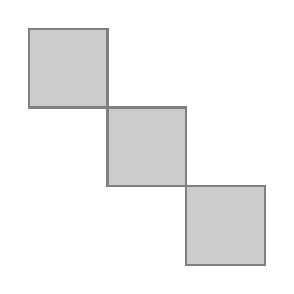
\begin{tikzpicture}
    [inner sep=5mm,
    place/.style={circle,draw=blue!50,fill=blue!20,thick},
    transition/.style={rectangle,draw=black!50,fill=black!20,thick}]
    \node at ( -2,2) [transition] {};
    \node at ( -1,1) [transition] {};
    \node at ( 0,0) [transition] {};
\end{tikzpicture}\end{pmatrix}$\\
\footnotesize{$\mathcal{H}=\mathcal{F}^0\oplus\mathcal{F}^1\oplus\cdots$\\不同的对角块分别对应不同粒子数的Fock空间,不同粒子数Fock空间的表示基相互正交,这是群论所要求的。}
\end{center}
同样的有完备性关系
\begin{equation*}
    \sum_{n_1,n_2,\cdots=0}^{1}|n_1,n_2,\cdots\rangle\langle n_1,n_2,\cdots|=1
\end{equation*}
这里我们希望引入产生算符$a_i^\dagger$。这些产生算符必须被定义成,两次连续作用后为0.进一步说,它们的顺序至关重要。我们如下定义产生算符$a_i^\dagger$
\begin{equation*}
    \begin{split}
        &S_-|i_1,i_2,\cdots,i_N\rangle=a_{i_1}^\dagger a_{i_2}^\dagger\cdots a_{i_N}^\dagger|0\rangle\\
        &S_-|i_2,i_1,\cdots,i_N\rangle=a_{i_2}^\dagger a_{i_1}^\dagger\cdots a_{i_N}^\dagger|0\rangle
    \end{split}
\end{equation*}
上下两式差一个负号,所以有反对易关系
\begin{equation*}
    \{a_i^\dagger,a_j^\dagger\}=0
\end{equation*}
这也意味着双占据态$(a_i^\dagger)^2=0$

为了方便我们定义对易子和反对易子
\begin{equation*}
    \begin{split}
        \{A,B\}&=[A,B]_{+}=AB+BA\\
        [A,B]&=[A,B]_-=AB-BA
    \end{split}
\end{equation*}
有了这些预先准备后,我们现在可以精确地处理公式。如果我们想要用占据数来表征各个粒子态就不得不选择一个特别地粒子态顺序。这个选择是任意的,但是一旦选定,随后所有的计算都必须按照选定的顺序。
\begin{equation*}
    |n_1,n_2\cdots\rangle=(a_1^\dagger)^{n_1}(a_2^\dagger)^{n_2}\cdots|0\rangle,\quad n_i=0,1
\end{equation*}
产生算符作用在占据数态上为
\begin{equation*}
    a_i^\dagger|\cdots,n_i,\cdots\rangle=(1-n_i)(-1)^{\sum_{j<i}n_j}|\cdots,n_i+1,\cdots\rangle
\end{equation*}
粒子数在产生算符作用下增加1,但是对于已经占据了粒子的状态,由于泡利不相容原理,产生算符作用应该是$0$,这点用$(1-n_i)$来保证$n_i=1$时为$0$. 值得注意,上式中$-1$来自于费米子反对称性。产生算符作用在$n_i$占据数态上需要越过$\sum_{j<i}n_j$次。
\begin{equation*}
    \begin{split}
        a_i^\dagger|\cdots,n_i,\cdots\rangle&=a_i^\dagger S_-|i_1,i_2,\cdots,i_N\rangle\\
        &=S_-a_i^\dagger|i_1,i_2,\cdots,i_N\rangle\\
        &=S_-|i\rangle\otimes|i_1,i_2,\cdots,i_N\rangle\\
        &=(-1)^{\sum_{j<i}n_j}S_-|i_1,i_2,\cdots,i,\cdots,i_N\rangle\\
        &=(1-n_i)(-1)^{\sum_{j<i}n_j}|\cdots,n_i+1,\cdots\rangle
    \end{split}
\end{equation*}
相同态的反对称化为$0$,这点用$(1-n_i)$来约束。同样的我们取厄米共轭得到
\begin{equation*}
    \langle\cdots,n_i,\cdots|a_i=(1-n_i)(-1)^{\sum_{j<i}n_j}\langle\cdots,n_i+1,\cdots|
\end{equation*}
用占据数态右乘上式
\begin{equation*}
    \langle\cdots,n_i,\cdots|a_i|\cdots,n_i',\cdots\rangle=(1-n_i)(-1)^{\sum_{j<i}n_j}\delta_{n_1,n_1'}\cdots\delta_{n_i+1,n_i'}\cdots
\end{equation*}
利用完备性关系
\begin{equation*}
    \sum_{n_1,n_2,\cdots}|n_1,n_2,\cdots\rangle\langle n_1,n_2,\cdots|=1
\end{equation*}
得到
\begin{equation*}
    \begin{split}
        a_i|n_1',\cdots,n_i',\cdots\rangle&=\sum_{n_1,\cdots,n_i,\cdots}|n_1,\cdots,n_i,\cdots\rangle\langle n_1,\cdots,n_i,\cdots|a_i|n_1',\cdots,n_i',\cdots\rangle\\
        &=\sum_{n_1,\cdots,n_i,\cdots}|n_1,\cdots,n_i,\cdots\rangle(1-n_i)(-1)^{\sum_{j<i}n_j}\delta_{n_1,n_1'}\delta_{n_2,n_2'}\cdots\delta_{n_i+1,n_i'}\cdots\\
        &=(2-n_i')n_i(-1)^{\sum_{j<i}n_j}|n_1',\cdots,n_i'-1,\cdots\rangle
    \end{split}
\end{equation*}
这里我们引入$n_i$以保证$n_i=0$时$Kronecker$符号为$0$,保证占据数非负。

总而言之,产生湮灭算符的关系为
\begin{equation*}
    \begin{split}
        a_i^\dagger|\cdots,n_i,\cdots\rangle&=(1-n_i)(-1)^{\sum_{j<i}n_j}|\cdots,n_i+1,\cdots\rangle\\
        a_i|\cdots,n_i,\cdots\rangle&=n_i(-1)^{\sum_{j<i}n_j}|\cdots,n_i-1,\cdots\rangle
    \end{split}
\end{equation*}
上式立马可得到
\begin{equation*}
    \begin{split}
        a_ia_i^\dagger|\cdots,n_i,\cdots\rangle&=(1-n_i)(-1)^{\sum_{j<in_j}}a_i|\cdots,n_i+1,\cdots\rangle\\
        &=(1-n_i)[(-1)^{\sum_{j<i}n_i}]^2(n_i+1)|\cdots,n_i,\cdots\rangle\\
        &=(1-n_i)|\cdots,n_i,\cdots\rangle\\
        a_i^\dagger a_i|\cdots,n_i,\cdots\rangle&=n_i(-1)^{\sum_{j<i}n_i}a_i^\dagger|\cdots,n_i-1,\cdots\rangle\\
        &=n_i[(-1)^{\sum_{j<i}n_i}]^2(2-n_i)|\cdots,n_i,\cdots\rangle\\
        &=n_i|\cdots,n_i,\cdots\rangle
    \end{split}
\end{equation*}
因为对于$n_i\in\{0,1\}$,我们有$n_i^2=n_i$和$[(-1)^{\sum_{j<i}n_j}]^2=1$. 由于上式的性质,我们定义占据态$|i\rangle$的粒子数算符为$n_i=a_i^\dagger a_i$。上面两式叠加得到
\begin{equation*}
    [a_i,a_i^\dagger]_+=1
\end{equation*}
对于$i\neq j$的情况
\begin{equation*}
    \begin{split}
        &[a_i,a_j^\dagger]_+|\cdots,n_i,n_j\cdots\rangle\\
        &=(1-n_j)(-1)^{\sum_{p<j}n_p}n_i(-1)^{\sum_{q,i}n_q}|\cdots,n_i,\cdots,n_j,\cdots\rangle\\
        &+n_i(-1)^{\sum_{q<i}n_q}(1-n_j)(-1)^{1+\sum_{p<j}n_p}|\cdots,n_i,\cdots,n_j,\cdots\rangle\\
        &=0
    \end{split}
\end{equation*}
同样的,对于$i\neq j$计算$[a_i,a_j]_+$也会出现相位相差$(-1)$���对于$i\neq j$的情况,由于$a_i^2=0$,所以$[a_i,a_i]=0$。综上,费米子反对易关系为
\begin{equation*}
    [a_i,a_j]_+=0,\quad[a_i^\dagger,a_j^\dagger]_+=0,\quad[a_i,a_j^\dagger]_+=\delta_{ij}
\end{equation*}
\subsubsection{单体算符和多体算符}
对于费米子系统,算符也可以表示成产生算符和湮灭算符。形式上和玻色子系统算符表示一样。现在我们要注意产生湮灭算符的顺序。
\begin{equation*}
    \sum_{\alpha}|i\rangle_{\alpha}\langle i|_\alpha=a_i^\dagger a_j
\end{equation*}
根据前一节证明过程,我们也能得到两体算符二次量子化形式:给定态$S_-|i_1,\cdots,i_N\rangle$,不失一般性,假设有$i_1<i_2<\cdots<i_N$
\begin{equation*}
    \begin{split}
        \sum_{\alpha}|i\rangle_\alpha\langle j|_\alpha S_-|i_1,i_2,\cdots,i_N\rangle&=S_-\sum_{\alpha}|i\rangle_{\alpha}\langle j|_\alpha |i_1,i_2,\cdots,i_N\rangle\\
        &=n_j(1-n_i)S_-|i_1,i_2,\cdots,i_N\rangle|_{j\to i}
    \end{split}
\end{equation*}
$j\to i$表示$j$态被$i$态替换。由于泡利不相容原理,当有两个$i$态时,应当为0,这点用$1-n_i$来保证。我们要注意,算符$\sum_{\alpha}|i\rangle_\alpha\langle j|_\alpha$的作用相当于$j$替换成$i$,但由于全反对称性,实际上交换次数会存在差异

对于$i\leq j$
\begin{equation*}
    \begin{split}
        S_-\sum_\alpha|i\rangle_\alpha\langle j|_\alpha|i_1\rangle\otimes\cdots|\tilde{i}\rangle\otimes|\tilde{j}\rangle\otimes|i_N\rangle&=(-1)^{\sum_{k<j}n_k}S_-\sum_\alpha|i\rangle_\alpha\otimes|i_1\rangle\otimes\cdots\otimes|\tilde{i}\rangle\otimes\cdots\otimes\langle j|_\alpha|\tilde{j}\rangle\otimes\cdots\otimes|i_N\rangle\\
        &=n_j(-1)^{\sum_{k\leq j}n_k}S_-|i\rangle\otimes|i_1\rangle\otimes\cdots\otimes|\tilde{i}\rangle\otimes\cdots\otimes|i_N\rangle\\
        &=n_j(1-n_i)(-1)^{\sum_{k\leq j}n_k+\sum_{k<i}n_k}|\cdots,n_i+1,\cdots,n_j-1,\cdots\rangle\\
    \end{split}
\end{equation*}
对于$i>j$
\begin{equation*}
    \begin{split}
        S_-\sum_\alpha|i\rangle_\alpha\langle j|_\alpha|i_1\rangle\otimes\cdots|\tilde{j}\rangle\otimes|\tilde{i}\rangle\otimes|i_N\rangle&=(-1)^{\sum_{k<j}n_k}S_-\sum_\alpha|i\rangle_\alpha\otimes|i_1\rangle\otimes\cdots\otimes\langle j|_\alpha|\tilde{j}\rangle\otimes\cdots\otimes|\tilde{i}\rangle\otimes\cdots\otimes|i_N\rangle\\
        &=n_j(-1)^{\sum_{k<j}n_k}S_-|i\rangle\otimes|i_1\rangle\otimes\cdots\otimes|\tilde{i}\rangle\otimes\cdots\otimes|i_N\rangle\\
        &=n_j(1-n_i)(-1)^{\sum_{k<j}n_k+\sum_{k<i}n_k-1}|\cdots,n_j-1,\cdots,n_i+1,\cdots\rangle
    \end{split}
\end{equation*}
我们观察$a_i^+a_j$作用在占据数态上
\begin{equation*}
    \begin{split}
        a_i^\dagger a_j|\cdots,n_i,\cdots,n_j,\cdots\rangle&=n_j(-1)^{\sum_{k<j}n_k}a_i^\dagger|\cdots,n_i,\cdots,n_j-1,\cdots\rangle\\
        &=n_j(1-n_i)(-1)^{\sum_{k<j}n_k+\sum_{k<i}n_k-\delta_{i>j}}|\cdots,n_i+1,\cdots,n_j-1,\cdots\rangle
    \end{split}
\end{equation*}
总而言之,对于玻色子和费米子,单体算符和两体算符写成
\begin{equation*}
    \begin{split}
        &T=\sum_{i,j}t_{ij}a_i^\dagger a_j\\
        &F=\frac{1}{2}\sum_{i,j,k,m}\langle i,j|f^{(2)}|k,m\rangle a_i^\dagger a_j^\dagger a_m a_k
    \end{split}
\end{equation*}
对于玻色子而言,$a_i$服从玻色对易关系,对于费米子而言$a_i$服从费米反对易关系。这样多体系统的哈密顿可以写成如下形式
\begin{equation*}
    H=\sum_{i,j}(t_{ij}+U_{ij})a_i^\dagger a_j+\frac{1}{2}\sum_{i,j,k,m}\langle i,j|f^{(2)}|k,m\rangle a_i^\dagger a_j^\dagger a_m a_k
\end{equation*}
特别注意,对于费米子而言,要注意两体算符对应湮灭算符的顺序。
\subsection{场算符}
我们考虑两组基底$\{|i\rangle\}$和$\{|\lambda\rangle\}$。很自然的会想到,$a_\lambda$和$a_i$之间是否有对应关系
\begin{equation*}
    |\lambda\rangle=\sum_{i}|i\rangle\langle i|\lambda\rangle,\quad a_i^\dagger|0\rangle=|i\rangle,\quad,a_\lambda^\dagger|0\rangle=|\lambda\rangle
\end{equation*}
算符$a_i^\dagger$在$|i\rangle$上产生一个粒子。因此,$\sum_{i}\langle i|\lambda\rangle a_i^\dagger$在态$|\lambda\rangle$上产生一个粒子。这样就有关系式
\begin{equation*}
    a_\lambda^\dagger=\sum_{i}\langle i|\lambda\rangle a_i^\dagger
\end{equation*}
上式去厄米共轭得到
\begin{equation*}
    a_\lambda=\sum_{i}\langle\lambda|i\rangle a_i
\end{equation*}
对于坐标表示来说
\begin{equation*}
    \langle x|i\rangle=\varphi_i(x)
\end{equation*}
其中$\varphi_i(x)$是单粒子波函数,产生湮灭算符对应于位置本征态下的叫做场算符。
\subsubsection{场算符}
场算符如下定义
\begin{equation*}
    \begin{split}
        \psi(x)&=\sum_{i}\varphi_i(x)a_i\\
        \psi^\dagger(x)&=\sum_{i}\varphi_i^*(x)a_i^\dagger
    \end{split}
\end{equation*}
场算符$\psi^\dagger(x)$在$x$位置产生一个粒子。场算符服从如下对易关系
\begin{equation*}
    \begin{split}
        [\psi(x),\psi(x')]_{\pm}&=0\\
        [\psi^\dagger(x),\psi^\dagger(x')]_{\pm}&=0\\
        [\psi(x),\psi^\dagger(x')]_{\pm}&=\sum_{i,j}\varphi_i(x)\varphi_j^*(x')[a_i,a_j^\dagger]=\sum_{i}\varphi_i(x)\varphi_i^*(x')=\delta(x-x')
    \end{split}
\end{equation*}
费米子对应于$(+)$,玻色子对应于$(-)$。

我们现在可以根据场算符的得到一些重要的算符表示
\begin{equation*}
    \begin{split}
        \sum_{i,j}a_i^\dagger T_{ij}a_j&=\sum_{i,j}a_i^\dagger\langle i|T|j\rangle a_j\\
        &=\sum_{i,j}\int d^3xd^3x' a_i^\dagger \langle i|x\rangle\langle x|T|x'\rangle\langle x'|j\rangle a_j\\
        &=\sum_{i,j}\int d^3xd^3x' a_i^\dagger\varphi_i^*(x)(-\frac{\hbar^2}{2m}\nabla^2)\delta(x-x')\varphi_j(x')a_j\\
        &=\int d^3x\psi^\dagger(x)(-\frac{\hbar^2}{2m}\nabla^2)\psi(x)=\frac{\hbar^2}{2m}\int d^3x\nabla\psi^\dagger(x)\nabla\psi(x)
    \end{split}
\end{equation*}
单体势
\begin{equation*}
    \begin{split}
        \sum_{i,j}a_i^\dagger U_{ij}a_j&=\sum_{i,j}\int d^3x a_i^\dagger\varphi_i^*(x)U(x)\varphi_j(x)a_j\\
        &=\int d^3x U(x)\psi^\dagger(x)\psi(x)
    \end{split}
\end{equation*}
两体相互作用
\begin{equation*}
    \begin{split}
        &\frac{1}{2}\sum_{i,j,k,m}\langle i,j|V|k,m\rangle a_i^\dagger a_j^\dagger a_m a_k\\
        &=\frac{1}{2}\sum_{i,j,k,m}\int d^3xd^3x'd^3x''d^3x'''\langle i,j|x,x'\rangle\langle x,x'|V|x'',x'''\rangle\langle x'',x'''|k,m\rangle a_i^\dagger a_j^\dagger a_m a_k\\
        &=\frac{1}{2}\sum_{i,j,k,m}\int d^3xd^3x'd^3x''d^3x'''\varphi_i^*(x)\varphi_j(x')V(x,x')\delta(x-x'')\delta(x'-x''')\varphi_k(x'')\varphi_m(x''')a_i^\dagger a_j^\dagger a_m a_k\\
        &=\frac{1}{2}\sum_{i,j,k,m}\int d^3xd^3x'\varphi_i^*(x)\varphi_j^*(x')V(x,x')\varphi_k(x)\varphi_m(x')a_i^\dagger a_j^\dagger a_m a_k\\
        &=\frac{1}{2}\int d^3xd^3x'V(x,x')\psi(x)^\dagger \psi^\dagger(x')\psi(x')\psi(x)
    \end{split}
\end{equation*}
系统哈密顿为
\begin{equation*}
    H=\int d^3x\left[\psi^\dagger(x)(-\frac{\hbar^2}{2m}\nabla^2)\psi(x)+U(x)\psi^\dagger(x)\psi(x)\right]+\frac{1}{2}\int d^3xd^3x'V(x,x')\psi^\dagger(x)\psi^\dagger(x')\psi(x')\psi(x)
\end{equation*}
粒子数密度算符定义为
\begin{equation*}
    n(x)=\delta(x-x_\alpha)
\end{equation*}
二次量子化表示为
\begin{equation*}
    \begin{split}
        n(x)&=\sum_{i,j}a_i^\dagger\langle i|\delta(x-x')|j\rangle a_j\\
        &=\sum_{i,j}\int d^3xd^3y a_i^\dagger\langle i|x\rangle\langle x|\delta(x-x')|y\rangle\langle y|j\rangle a_j\\
        &=\sum_{i,j}\int d^3xd^3y a_i^\dagger\varphi_i^*(x)\delta(x-x')\delta(x-y)\varphi_j(y)a_j\\
        &=\sum_{i,j}\int d^3ya_i^\dagger\varphi_i^*(y)\delta(y-x')\varphi_i(y)a_j\\
        &=\sum_{i,j}\int d^3ya_i^\dagger\varphi_i^*(y)\delta(x-y)\varphi_i(y)a_j\\
        &=\int d^3y\psi^\dagger(y)\delta(x-y)\psi(y)\\
        &=\psi^\dagger(x)\psi(x)
    \end{split}
\end{equation*}
总粒子数算符
\begin{equation*}
    N=\int d^3xn(x)=\int d^3x\psi^\dagger(x)\psi(x)
\end{equation*}
从形式上来看,多粒子系统的粒子密度算符看起来像单粒子在态$\psi(x)$下的概率密度。然而,这种类比仅仅只是形式上的,因为前者是算符,后者是复变函数。这个形式上的对应被叫做二次量子化,因为场算符算符可以通过替换单粒子密度波函数$\psi(x)$为算符$\hat{\psi}(x)$来获得。这种对应使我们能写出流密度算符
\begin{equation*}
    j(x)=\frac{\hbar}{2im}[\psi^\dagger(x)\nabla\psi(x)-(\nabla\psi^\dagger(x))\psi(x)]
\end{equation*}
动能项形式上类似于单粒子动能的平均期望值,然而其中波函数被场算符所代替。

值得注意由场算符表示的算符可以直接得到,例如单粒子密度算符
\begin{equation*}
    \int d^3\xi d^3\xi'\psi^\dagger\langle\xi|\delta(x-\hat{\xi})|\xi'\rangle\psi(\xi')=\psi^\dagger(x)\psi(x)
\end{equation*}
其中$\hat{\xi}$是单粒子坐标算符。一般而言,对于$k$粒子算符$V_k$
\begin{equation*}
    \int d^3\xi_1\cdots d^3\xi_kd^3\xi_1'\cdots d^3\xi_k'\psi^\dagger(\xi_1)\cdots\psi^\dagger(\xi_k)\langle\xi_1\xi_2\cdots\xi_k|V_k|\xi_1'\xi_2'\cdots\xi_k'\rangle\psi(\xi_k')\cdots\psi(\xi_1')
\end{equation*}
\subsubsection{场方程}
场算符$\psi(x,t)$在海森堡表象下的形式为
\begin{equation*}
    \psi(x,t)=e^{iHt/\hbar}\psi(x,0)e^{-iHt/\hbar}
\end{equation*}
对于两体系统的哈密顿,有运动方程
\begin{equation*}
    i\hbar\frac{\partial}{\partial t}\psi(x,t)=\left[-\frac{\hbar^2}{2m}\nabla^2+U(x)\right]\psi(x,t)+\int d^3x'\psi^\dagger(x',t)V(x,x')\psi(x',t)\psi(x,t)
\end{equation*}
这回死一个非线性薛定谔方程,也叫二次量子化薛定谔方程。我们先证明上式
\begin{proof}
    首先从海森堡方程开始
    \begin{equation*}
        i\hbar\frac{\partial}{\partial t}\psi(x,t)=-[H,\psi(x,t)]=-e^{iHt/\hbar}[H,\psi(x,0)]e^{iHt/\hbar}
    \end{equation*}
    利用关系式
    \begin{equation*}
        [AB,C]_{\pm}=A[B,C]_{\pm}\mp[A,C]_{\pm}B
    \end{equation*}
    对于动能项
    \begin{equation*}
        \begin{split}
            &\int d^3x'\frac{\hbar^2}{2m}[\nabla'\psi^\dagger(x')\nabla'\psi(x'),\psi(x)]\\
            &=\int d^3x'\frac{\hbar^2}{2m}(-\nabla'\delta(x'-x))\nabla'\psi(x')=\frac{\hbar^2}{2m}\nabla^2\psi(x)
        \end{split}
    \end{equation*}
    对于单粒子势能项
    \begin{equation*}
        \begin{split}
            &\int d^3x'U(x')[\psi^\dagger(x')\psi(x'),\psi(x)]\\
            &=\int d^3x'U(x')(-\delta(x'-x)\psi(x'))=-U(x)\psi(x)
        \end{split}
    \end{equation*}
    两体相互作用项
    \begin{equation*}
        \begin{split}
            &\frac{1}{2}\left[\int d^3x'd^3x''\psi^\dagger(x')\psi^\dagger(x'')V(x',x'')\psi(x'')\psi(x'),\psi(x)\right]\\
            &=\frac{1}{2}\int d^3x'd^3x''[\psi^\dagger(x')\psi^\dagger(x''),\psi(x)]V(x',x'')\psi(x'')\psi(x')\\
            &=\frac{1}{2}\int d^3x'd^3x''[\pm\delta(x''-x)\psi^\dagger(x')-\delta(x'-x)\psi^\dagger(x'')]V(x',x'')\psi(x'')\psi(x')\\
            &=-\int d^3x\psi^\dagger(x')V(x,x')\psi(x')\psi(x)
        \end{split}
    \end{equation*}
    上述第二行应用了对易展开公式,在第三行应用了关系式$\psi(x'')\psi(x')=\mp\psi(x')\psi(x'')$以及对称性$V(x,x')=V(x',x)$. 这样就证明了场方程
\end{proof}
同样的,可以得到伴随场方程
\begin{equation*}
    i\hbar\psi^\dagger(x,t)=-\left[-\frac{\hbar^2}{2m}\nabla^2+U(x)\right]\psi^\dagger(x,t)-\int d^3x'\psi^\dagger(x,t)\psi^\dagger(x',t)V(x,x')\psi(x',t)
\end{equation*}
这里我们假设了$V^*(x,x')=V(x,x')$。场方程和伴随场方程分别左乘$\psi^\dagger(x,t)$和右乘$\psi(x,t)$,相减得到
\begin{equation*}
    \dot{n}(x,t)=(\psi^\dagger\dot{\psi}+\dot{\psi}^\dagger\psi)=-\frac{\hbar}{2mi}[\psi^\dagger\nabla^2\psi-(\nabla^2\psi^\dagger)\psi]
\end{equation*}
这样就得到了连续性方程
\begin{equation*}
    \dot{n}(x)=-\nabla\cdot J(x)
\end{equation*}
这里$J(x)$是粒子流密度。方程是粒子数密度的连续性方程。
\subsection{动量表象}
在平以不变系统里,动量表象是一个特别方便的表象。我们考虑在一个正方形盒子里的归一化,系统三维长度分别为$L_x,L_y,L_z$。动量本征函数用归一化平面波来表示。
\begin{equation*}
    \varphi_k(x)=\frac{e^{ikx}}{\sqrt{V}}
\end{equation*}
体积$V=L_xL_yL_z$. 通过假设周期性边界条件
\begin{equation*}
    e^{ik(x+L_x)}=e^{ikx}
\end{equation*}
允许的波矢$k$约束为
\begin{equation*}
    k=2\pi\left(\frac{n_x}{L_x},\frac{n_y}{L_y},\frac{n_z}{L_z}\right),\quad n_x=0,\pm1,\cdots,n_y=0,\pm1,\cdots,n_z=0,\pm1,\cdots
\end{equation*}
本征函数$\varphi_k(x)$满足正交归一关系
\begin{equation*}
    \int d^3x\varphi_k^*(x)\varphi_{k'}(x)=\delta_{k,k'}
\end{equation*}



\end{document} 